% Options for packages loaded elsewhere
% Options for packages loaded elsewhere
\PassOptionsToPackage{unicode}{hyperref}
\PassOptionsToPackage{hyphens}{url}
\PassOptionsToPackage{dvipsnames,svgnames,x11names}{xcolor}
%
\documentclass[
  english,
  a4paper,
  DIV=11,
  numbers=noendperiod]{scrreprt}
\usepackage{xcolor}
\usepackage[top=24mm,bottom=24mm,left=24mm,right=24mm]{geometry}
\usepackage{amsmath,amssymb}
\setcounter{secnumdepth}{5}
\usepackage{iftex}
\ifPDFTeX
  \usepackage[T1]{fontenc}
  \usepackage[utf8]{inputenc}
  \usepackage{textcomp} % provide euro and other symbols
\else % if luatex or xetex
  \usepackage{unicode-math} % this also loads fontspec
  \defaultfontfeatures{Scale=MatchLowercase}
  \defaultfontfeatures[\rmfamily]{Ligatures=TeX,Scale=1}
\fi
\usepackage{lmodern}
\ifPDFTeX\else
  % xetex/luatex font selection
\fi
% Use upquote if available, for straight quotes in verbatim environments
\IfFileExists{upquote.sty}{\usepackage{upquote}}{}
\IfFileExists{microtype.sty}{% use microtype if available
  \usepackage[]{microtype}
  \UseMicrotypeSet[protrusion]{basicmath} % disable protrusion for tt fonts
}{}
\makeatletter
\@ifundefined{KOMAClassName}{% if non-KOMA class
  \IfFileExists{parskip.sty}{%
    \usepackage{parskip}
  }{% else
    \setlength{\parindent}{0pt}
    \setlength{\parskip}{6pt plus 2pt minus 1pt}}
}{% if KOMA class
  \KOMAoptions{parskip=half}}
\makeatother
% Make \paragraph and \subparagraph free-standing
\makeatletter
\ifx\paragraph\undefined\else
  \let\oldparagraph\paragraph
  \renewcommand{\paragraph}{
    \@ifstar
      \xxxParagraphStar
      \xxxParagraphNoStar
  }
  \newcommand{\xxxParagraphStar}[1]{\oldparagraph*{#1}\mbox{}}
  \newcommand{\xxxParagraphNoStar}[1]{\oldparagraph{#1}\mbox{}}
\fi
\ifx\subparagraph\undefined\else
  \let\oldsubparagraph\subparagraph
  \renewcommand{\subparagraph}{
    \@ifstar
      \xxxSubParagraphStar
      \xxxSubParagraphNoStar
  }
  \newcommand{\xxxSubParagraphStar}[1]{\oldsubparagraph*{#1}\mbox{}}
  \newcommand{\xxxSubParagraphNoStar}[1]{\oldsubparagraph{#1}\mbox{}}
\fi
\makeatother

\usepackage{color}
\usepackage{fancyvrb}
\newcommand{\VerbBar}{|}
\newcommand{\VERB}{\Verb[commandchars=\\\{\}]}
\DefineVerbatimEnvironment{Highlighting}{Verbatim}{commandchars=\\\{\}}
% Add ',fontsize=\small' for more characters per line
\usepackage{framed}
\definecolor{shadecolor}{RGB}{241,243,245}
\newenvironment{Shaded}{\begin{snugshade}}{\end{snugshade}}
\newcommand{\AlertTok}[1]{\textcolor[rgb]{0.68,0.00,0.00}{#1}}
\newcommand{\AnnotationTok}[1]{\textcolor[rgb]{0.37,0.37,0.37}{#1}}
\newcommand{\AttributeTok}[1]{\textcolor[rgb]{0.40,0.45,0.13}{#1}}
\newcommand{\BaseNTok}[1]{\textcolor[rgb]{0.68,0.00,0.00}{#1}}
\newcommand{\BuiltInTok}[1]{\textcolor[rgb]{0.00,0.23,0.31}{#1}}
\newcommand{\CharTok}[1]{\textcolor[rgb]{0.13,0.47,0.30}{#1}}
\newcommand{\CommentTok}[1]{\textcolor[rgb]{0.37,0.37,0.37}{#1}}
\newcommand{\CommentVarTok}[1]{\textcolor[rgb]{0.37,0.37,0.37}{\textit{#1}}}
\newcommand{\ConstantTok}[1]{\textcolor[rgb]{0.56,0.35,0.01}{#1}}
\newcommand{\ControlFlowTok}[1]{\textcolor[rgb]{0.00,0.23,0.31}{\textbf{#1}}}
\newcommand{\DataTypeTok}[1]{\textcolor[rgb]{0.68,0.00,0.00}{#1}}
\newcommand{\DecValTok}[1]{\textcolor[rgb]{0.68,0.00,0.00}{#1}}
\newcommand{\DocumentationTok}[1]{\textcolor[rgb]{0.37,0.37,0.37}{\textit{#1}}}
\newcommand{\ErrorTok}[1]{\textcolor[rgb]{0.68,0.00,0.00}{#1}}
\newcommand{\ExtensionTok}[1]{\textcolor[rgb]{0.00,0.23,0.31}{#1}}
\newcommand{\FloatTok}[1]{\textcolor[rgb]{0.68,0.00,0.00}{#1}}
\newcommand{\FunctionTok}[1]{\textcolor[rgb]{0.28,0.35,0.67}{#1}}
\newcommand{\ImportTok}[1]{\textcolor[rgb]{0.00,0.46,0.62}{#1}}
\newcommand{\InformationTok}[1]{\textcolor[rgb]{0.37,0.37,0.37}{#1}}
\newcommand{\KeywordTok}[1]{\textcolor[rgb]{0.00,0.23,0.31}{\textbf{#1}}}
\newcommand{\NormalTok}[1]{\textcolor[rgb]{0.00,0.23,0.31}{#1}}
\newcommand{\OperatorTok}[1]{\textcolor[rgb]{0.37,0.37,0.37}{#1}}
\newcommand{\OtherTok}[1]{\textcolor[rgb]{0.00,0.23,0.31}{#1}}
\newcommand{\PreprocessorTok}[1]{\textcolor[rgb]{0.68,0.00,0.00}{#1}}
\newcommand{\RegionMarkerTok}[1]{\textcolor[rgb]{0.00,0.23,0.31}{#1}}
\newcommand{\SpecialCharTok}[1]{\textcolor[rgb]{0.37,0.37,0.37}{#1}}
\newcommand{\SpecialStringTok}[1]{\textcolor[rgb]{0.13,0.47,0.30}{#1}}
\newcommand{\StringTok}[1]{\textcolor[rgb]{0.13,0.47,0.30}{#1}}
\newcommand{\VariableTok}[1]{\textcolor[rgb]{0.07,0.07,0.07}{#1}}
\newcommand{\VerbatimStringTok}[1]{\textcolor[rgb]{0.13,0.47,0.30}{#1}}
\newcommand{\WarningTok}[1]{\textcolor[rgb]{0.37,0.37,0.37}{\textit{#1}}}

\usepackage{longtable,booktabs,array}
\newcounter{none} % for unnumbered tables
\usepackage{calc} % for calculating minipage widths
% Correct order of tables after \paragraph or \subparagraph
\usepackage{etoolbox}
\makeatletter
\patchcmd\longtable{\par}{\if@noskipsec\mbox{}\fi\par}{}{}
\makeatother
% Allow footnotes in longtable head/foot
\IfFileExists{footnotehyper.sty}{\usepackage{footnotehyper}}{\usepackage{footnote}}
\makesavenoteenv{longtable}
\usepackage{graphicx}
\makeatletter
\newsavebox\pandoc@box
\newcommand*\pandocbounded[1]{% scales image to fit in text height/width
  \sbox\pandoc@box{#1}%
  \Gscale@div\@tempa{\textheight}{\dimexpr\ht\pandoc@box+\dp\pandoc@box\relax}%
  \Gscale@div\@tempb{\linewidth}{\wd\pandoc@box}%
  \ifdim\@tempb\p@<\@tempa\p@\let\@tempa\@tempb\fi% select the smaller of both
  \ifdim\@tempa\p@<\p@\scalebox{\@tempa}{\usebox\pandoc@box}%
  \else\usebox{\pandoc@box}%
  \fi%
}
% Set default figure placement to htbp
\def\fps@figure{htbp}
\makeatother



\ifLuaTeX
\usepackage[bidi=basic,shorthands=off]{babel}
\else
\usepackage[bidi=default,shorthands=off]{babel}
\fi
\ifLuaTeX
  \usepackage{selnolig} % disable illegal ligatures
\fi


\setlength{\emergencystretch}{3em} % prevent overfull lines

\providecommand{\tightlist}{%
  \setlength{\itemsep}{0pt}\setlength{\parskip}{0pt}}



 


\KOMAoption{captions}{tableheading}
\makeatletter
\@ifpackageloaded{tcolorbox}{}{\usepackage[skins,breakable]{tcolorbox}}
\@ifpackageloaded{fontawesome5}{}{\usepackage{fontawesome5}}
\definecolor{quarto-callout-color}{HTML}{909090}
\definecolor{quarto-callout-note-color}{HTML}{0758E5}
\definecolor{quarto-callout-important-color}{HTML}{CC1914}
\definecolor{quarto-callout-warning-color}{HTML}{EB9113}
\definecolor{quarto-callout-tip-color}{HTML}{00A047}
\definecolor{quarto-callout-caution-color}{HTML}{FC5300}
\definecolor{quarto-callout-color-frame}{HTML}{acacac}
\definecolor{quarto-callout-note-color-frame}{HTML}{4582ec}
\definecolor{quarto-callout-important-color-frame}{HTML}{d9534f}
\definecolor{quarto-callout-warning-color-frame}{HTML}{f0ad4e}
\definecolor{quarto-callout-tip-color-frame}{HTML}{02b875}
\definecolor{quarto-callout-caution-color-frame}{HTML}{fd7e14}
\makeatother
\makeatletter
\@ifpackageloaded{bookmark}{}{\usepackage{bookmark}}
\makeatother
\makeatletter
\@ifpackageloaded{caption}{}{\usepackage{caption}}
\AtBeginDocument{%
\ifdefined\contentsname
  \renewcommand*\contentsname{Table of contents}
\else
  \newcommand\contentsname{Table of contents}
\fi
\ifdefined\listfigurename
  \renewcommand*\listfigurename{List of Figures}
\else
  \newcommand\listfigurename{List of Figures}
\fi
\ifdefined\listtablename
  \renewcommand*\listtablename{List of Tables}
\else
  \newcommand\listtablename{List of Tables}
\fi
\ifdefined\figurename
  \renewcommand*\figurename{Figure}
\else
  \newcommand\figurename{Figure}
\fi
\ifdefined\tablename
  \renewcommand*\tablename{Table}
\else
  \newcommand\tablename{Table}
\fi
}
\@ifpackageloaded{float}{}{\usepackage{float}}
\floatstyle{ruled}
\@ifundefined{c@chapter}{\newfloat{codelisting}{h}{lop}}{\newfloat{codelisting}{h}{lop}[chapter]}
\floatname{codelisting}{Listing}
\newcommand*\listoflistings{\listof{codelisting}{List of Listings}}
\makeatother
\makeatletter
\makeatother
\makeatletter
\@ifpackageloaded{caption}{}{\usepackage{caption}}
\@ifpackageloaded{subcaption}{}{\usepackage{subcaption}}
\makeatother
\usepackage{bookmark}
\IfFileExists{xurl.sty}{\usepackage{xurl}}{} % add URL line breaks if available
\urlstyle{same}
% fallback for those not using the hyperref driver hyperxmp:
\makeatletter
\@ifundefined{xmpquote}{\newcommand{\xmpquote}[1]{#1}}{}
\makeatother
\hypersetup{
  pdftitle={From Episodes to Revisable Concepts},
  pdfauthor={Danny Ruchtie},
  pdflang={en},
  colorlinks=true,
  linkcolor={blue},
  filecolor={Maroon},
  citecolor={Blue},
  urlcolor={Blue},
  pdfcreator={LaTeX via pandoc}}


\title{From Episodes to Revisable Concepts}
\usepackage{etoolbox}
\makeatletter
\providecommand{\subtitle}[1]{% add subtitle to \maketitle
  \apptocmd{\@title}{\par {\large #1 \par}}{}{}
}
\makeatother
\subtitle{The Experience Learning Layer for Evidence-Grounded Learning
in Language Agents}
\author{Danny Ruchtie}
\date{2026-08-09}
\begin{document}
\maketitle

\renewcommand*\contentsname{Table of contents}
{
\setcounter{tocdepth}{2}
\tableofcontents
}

\bookmarksetup{startatroot}

\chapter*{Abstract}\label{abstract}
\addcontentsline{toc}{chapter}{Abstract}

\markboth{Abstract}{Abstract}

\begin{tcolorbox}[enhanced jigsaw, arc=.35mm, bottomrule=.15mm, bottomtitle=1mm, breakable, colback=white, colbacktitle=quarto-callout-note-color!10!white, colframe=quarto-callout-note-color-frame, coltitle=black, left=2mm, leftrule=.75mm, opacityback=0, opacitybacktitle=0.6, rightrule=.15mm, title=\textcolor{quarto-callout-note-color}{\faInfo}\hspace{0.5em}{Living working draft v0.6 - 9 August 2026}, titlerule=0mm, toprule=.15mm, toptitle=1mm]

Version 0.6 sharpens the contribution boundary after a review of current
agent-memory, experience-learning, provenance, belief-revision, and
evaluation research. It defines one confirmatory outcome, explicit
success and failure gates, a benchmark-first implementation plan, and a
narrower ELL-Core. Earlier drafts remain available through Git history.

\textbf{Research status.} This document is a working architecture paper
and preregistered evaluation plan. It defines the proposed system,
hypotheses, data model, implementation contract, and experiments. It
does not report empirical results. Results will be added only after the
open implementation and evaluation harness can reproduce them.

\end{tcolorbox}

Large language model agents can store and retrieve previous
interactions, yet retrieval alone does not establish that an agent has
learned from experience. Learning requires a system to identify patterns
across episodes, distinguish observations from hypotheses, form reusable
concepts, apply those concepts in new situations, and revise them when
later evidence disagrees. Recent agent-memory research has introduced
reflection, experience-derived insights, workflow induction, dynamic
memory graphs, semantic and procedural memory, schema induction, and
temporally grounded updates. The remaining challenge is therefore not
simply to add another memory store, but to make the transition from
experience to general knowledge explicit, inspectable, revisable, and
directly measurable.

This paper proposes the Experience Learning Layer (ELL), an open,
model-independent architecture positioned between an agent's experience
history and its decision process. ELL preserves raw episodes in an
append-only store, creates typed associations between them, represents
reflections as provisional interpretations, and promotes compatible
reflections into versioned concepts. Each concept records its scope,
supporting evidence, counterevidence, confidence, temporal validity,
lineage, and observed utility. Concepts can be corroborated, contested,
revised, superseded, or retired without erasing their evidential
history.

The system north star is to give any AI a natural, evolving intuition
about the user or organisation: grounded in experience, economical to
use, sensitive to change, explainable when inspected, and always under
user control.

Here intuition is neither anthropomorphism nor a new memory category. It
names an emergent system capability produced by evidence-grounded
compression, prediction, association, relevance selection, temporal
adaptation, and outcome feedback. At use time, ELL should supply a
compact intuition packet rather than dump raw history into a model,
while retaining links that permit inspection, correction, deletion, and
uncertainty-aware expansion.

The paper contributes a minimal typed architecture, a concept-lifecycle
protocol, an evidence ledger, a controlled benchmark, and an
evaluation-first implementation plan. It does not claim that reflection,
abstraction, provenance, temporal memory, or external memory is
individually novel. Its primary confirmatory claim is narrower: under
matched model and total-compute conditions, an evidence-governed concept
layer should improve transfer to structurally related but lexically
different tasks over the strongest eligible non-parametric baseline,
while satisfying preregistered guardrails for unsupported
generalisation, evidence quality, adaptation, governance, and cost. If
it does not, the concept layer is not justified.

\emph{Keywords: agent memory; experiential learning; reflection; concept
formation; semantic memory; continual learning; provenance; language
agents; open source}

\begin{figure}[H]

{\centering \pandocbounded{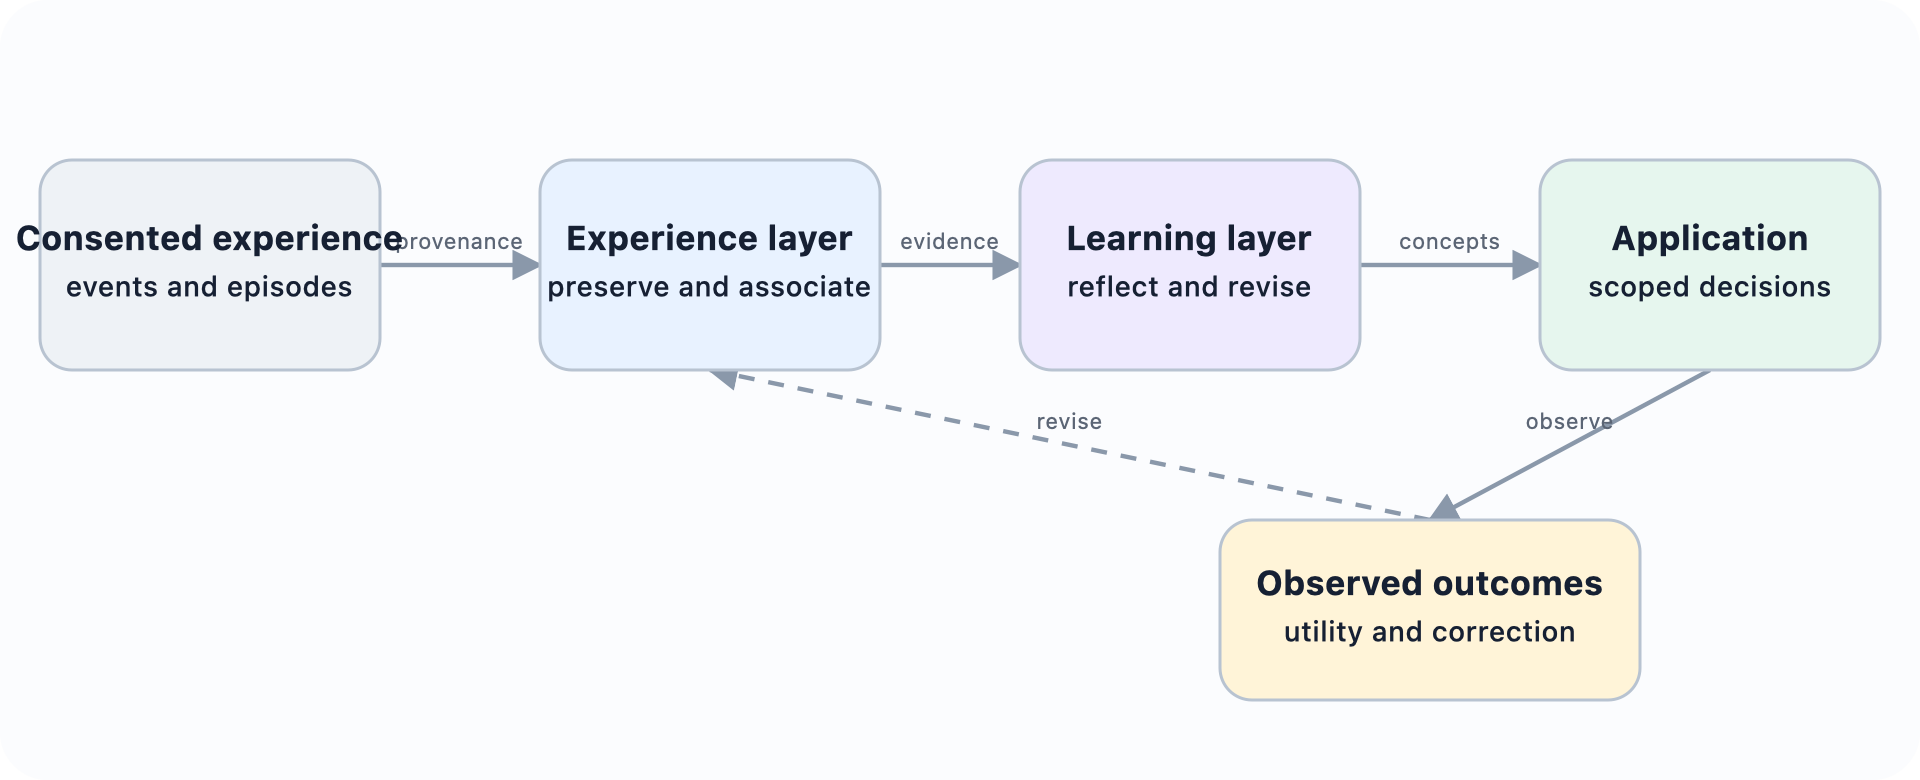
\includegraphics[keepaspectratio]{chapters/assets/diagrams/ell-overview.png}}

}

\caption{Where the Experience Learning Layer sits}

\end{figure}%

\bookmarksetup{startatroot}

\chapter{Introduction}\label{introduction}

A language agent can remember an earlier event without learning anything
general from it. A retrieval system may surface five examples of the
same failure, yet the agent may still repeat that failure because the
episodes have never been converted into a reusable and appropriately
scoped principle. This distinction matters as agents move from
single-turn assistance toward persistent collaboration, long-running
tasks, and multi-session interaction.

The intended user experience is stronger than factual continuity. An AI
should understand conversational shorthand, surface relevant context
just in time, generalise usefully across related situations, notice when
a previous pattern has changed, correct itself rapidly, and express
calibrated uncertainty. Explanations should be available when requested
without forcing provenance detail into every interaction. These
behaviours constitute the proposed operational meaning of an evolving
intuition; they do not imply consciousness, personhood, or a simulation
of human cognition.

The first generation of agent-memory systems established that external
memory could improve continuity beyond a model's context window.
Generative Agents stored observations, ranked them for retrieval, and
periodically synthesised higher-level reflections that influenced later
plans (Park et al.~2023). Reflexion used textual feedback about prior
attempts as a non-parametric learning signal (Shinn et al.~2023). ExpeL
extracted natural-language insights from collections of task experiences
and reused both insights and successful trajectories at inference time
(Zhao et al.~2024). MemGPT approached the problem as virtual context
management, allowing an agent to move information between limited
working context and external storage (Packer et al.~2023). CoALA
organised these developments within a broader cognitive architecture
containing working, episodic, semantic, and procedural memory (Sumers et
al.~2024).

Subsequent systems have increasingly abstracted experience rather than
merely retrieving it. Voyager accumulated reusable executable skills (G.
Wang et al.~2023). Agent Workflow Memory induced recurring action
routines from prior trajectories (Z. Z. Wang et al.~2025). A-MEM
dynamically linked and revised memory notes as new information arrived
(Xu et al.~2025). Reflective Memory Management used prospective and
retrospective reflection to improve memory granularity and retrieval (Z.
Tan et al.~2025). Hindsight separates world, experience, observation,
and opinion networks and allows opinions to evolve with confidence
(Latimer et al.~2026). More recent architectures explicitly construct
schemas, concepts, semantic knowledge, or procedural knowledge from
episodes, including DCPM, GAAMA, and PlugMem (Fei et al.~2026; Paul,
Sharma, and Sareen 2026; Yang et al.~2026). A recent survey describes
this field-wide progression as storage, reflection, and experience
abstraction (Luo et al.~2026).

This rapid progress changes the research question. It is no longer
defensible to claim that transforming episodes into abstractions is
itself novel. Nor are provenance, non-monotonic belief revision,
temporal validity, or dependency-based retraction new in isolation. The
more precise question is: Does combining these ideas in an external
language-agent learning layer produce a measurable advantage over
simpler memory methods, and can that advantage survive explicit safety,
adaptation, and cost constraints?

ELL addresses this question by separating four objects that are often
collapsed into one textual memory:

\begin{enumerate}
\def\labelenumi{\arabic{enumi}.}
\tightlist
\item
  An episode records what occurred in a specific context.
\item
  A reflection is a provisional interpretation of one or more episodes.
\item
  A concept is a reusable proposition or strategy supported by multiple
  reflections and episodes.
\item
  An application outcome records whether using a concept helped in a
  later situation.
\end{enumerate}

The separation is important because a plausible explanation is not
automatically reliable knowledge. Suppose a project proposal is rejected
after stakeholders were consulted late. A reflection may state that late
stakeholder involvement caused the rejection. That is a useful
hypothesis, but a single episode does not justify a universal rule. A
concept should only be promoted after corroborating cases, explicit
checks for counterexamples, and a scope statement such as
``cross-functional initiatives with external implementation
dependencies.'' New evidence may later narrow, challenge, or replace it.

ELL treats every concept as a versioned claim rather than a timeless
fact. The system retains the episodes that support it, episodes that
contradict it, the contexts in which it has been applied, and the
outcomes of those applications. This makes concept formation inspectable
and enables evaluation at the level where learning is claimed to occur.

The architecture is inspired by, but does not attempt to reproduce,
human memory. Tulving's distinction between episodic and semantic memory
motivates the separation between event-specific records and general
knowledge (Tulving 1972). Complementary Learning Systems theory
motivates a fast episodic path and a slower consolidation path that
integrates common structure across experiences (McClelland, McNaughton,
and O'Reilly 1995; Kumaran, Hassabis, and McClelland 2016). Bartlett's
account of reconstructive remembering provides a warning as much as an
inspiration: abstraction can impose existing schemas on ambiguous
experience and thereby distort it (Bartlett 1932). For this reason, ELL
preserves provenance, counterevidence, and reversible revisions.

\section{Scope}\label{scope}

ELL is an external learning layer. It does not update the parameters of
the underlying language model. It does not prescribe how raw activity is
captured from calendars, files, screens, sensors, or chat applications.
It starts after an application has produced a canonical stream of
consented experience records. It is designed to support conversation
histories, task trajectories, product-work records, and other event
streams through a shared schema.

The confirmatory research scope is deliberately narrower than a complete
personal-intelligence system. ELL-Core contains only source evidence,
episodes, provisional reflections, versioned concepts, evidence links,
application receipts, and outcomes. It focuses on:

\begin{itemize}
\tightlist
\item
  association between episodes;
\item
  reflection over individual and grouped episodes;
\item
  concept formation and consolidation;
\item
  application of concepts to later decisions;
\item
  revision after new evidence and outcomes;
\item
  direct evaluation of concept quality and transfer.
\end{itemize}

Perception, multimodal capture, large-scale identity resolution,
autonomous skill evolution, learned memory-operation policies, neural
memory, production provider integrations, and parametric fine-tuning are
outside the first confirmatory study. They remain possible follow-on
experiments only after ELL-Core clears its success gates.

\section{Contributions}\label{contributions}

This working paper specifies five intended contributions.

A minimal experience-to-concept contract. It defines distinct schemas
and operations for evidence, episodes, reflections, concepts,
applications, and outcomes without requiring a graph, vector database,
or hosted memory provider.

An evidence-grounded concept lifecycle. Concepts move through explicit
states---proposed, corroborated, contested, revised, superseded, and
retired---while retaining lineage and provenance.

A separation between confidence and eloquence. Concept confidence is
computed from observable evidence, contradiction, diversity, and outcome
history rather than accepted directly from an LLM's self-reported
certainty.

A confirmatory evaluation protocol. One primary transfer outcome is
paired with preregistered epistemic, adaptation, governance, and cost
guardrails. Component metrics diagnose why the result occurred; they do
not substitute for behavioural improvement.

An evaluation-first open implementation plan. The benchmark and simple
baselines are built before the concept engine. Versioned releases will
include schemas, prompts, configurations, generators, evaluation
scripts, raw receipts, and paper sources under permissive licences, with
reproducibility runs using open-weight models.

\bookmarksetup{startatroot}

\chapter{Problem Definition}\label{problem-definition}

\section{Experience learning}\label{experience-learning}

Let an agent encounter an ordered experience stream E=\{e1 ,e2
,\ldots,en\}.

Each episode ei contains a time-bounded record of context, observation,
action, outcome, source, and metadata. Given this stream, an
experience-learning system should produce a set of concepts C that
improve decisions on future situations while remaining grounded in the
episodes from which they were induced.

The goal is not to compress the entire history into a shorter text.
Compression can preserve frequent information while losing exceptions,
causal uncertainty, temporal change, and source identity. The desired
output is a set of claims or strategies with explicit conditions and
evidence.

A concept is useful only if it satisfies several properties:

\begin{itemize}
\item
  Grounded: its support can be traced to specific episodes and
  reflections.
\item
  General: it applies beyond a single remembered case.
\item
  Scoped: it states where it is expected to apply and where it may not.
\item
  Revisable: contradictory evidence can change its status or content.
\item
  Actionable: it can affect a later response, plan, or decision.
\item
  Measurable: its correctness and utility can be evaluated
  independently.
\end{itemize}

\section{Failure modes addressed}\label{failure-modes-addressed}

ELL is designed around seven common failure modes.

Episode replay without abstraction. Relevant cases are retrieved, but no
reusable principle is formed.

Premature generalisation. A single salient episode becomes a broad rule.

Self-confirming reflection. Once a reflection is stored, later retrieval
favours evidence that agrees with it.

Context collapse. A concept loses the conditions under which it was
valid.

Temporal staleness. New evidence changes what is true, but the old
concept continues to guide behaviour.

Provenance loss. A generated statement can no longer be connected to the
experience that justified it.

Behavioural ambiguity. A system claims to have learned because it stored
a summary, without showing improved transfer or decision quality.

\section{Research questions and claim
hierarchy}\label{research-questions-and-claim-hierarchy}

The first empirical study will answer five questions, but they do not
have equal confirmatory status.

RQ1 --- Separation. Does representing reflections as provisional objects
before concept consolidation reduce unsupported generalisation compared
with direct episode-to-rule summarisation?

RQ2 --- Revision. Do explicit counterevidence, temporal validity, and
versioned lifecycle states improve adaptation when the underlying
pattern changes?

RQ3 --- Transfer. Do consolidated concepts improve performance on new
situations that share latent structure but differ in wording and surface
details?

RQ4 --- Efficiency. Can compact concepts plus selected source episodes
match or improve downstream performance while using less retrieval
context than episode-only methods?

RQ5 --- Intuition quality. Can a compact, uncertainty-aware intuition
packet improve shorthand understanding, just-in-time relevance, change
detection, and rapid correction compared with no-memory, raw-history,
and ordinary retrieval-augmented generation baselines?

RQ3 is the primary confirmatory question. RQ1 is its epistemic safety
guardrail: a transfer gain does not count if it is purchased through
materially greater unsupported generalisation. RQ2 and RQ4 are secondary
mechanism and efficiency questions. RQ5 is an exploratory product-facing
question and cannot establish the core claim by itself.

\section{Hypotheses}\label{hypotheses}

H1. ELL will produce higher concept-scope accuracy and lower
overgeneralisation than a direct insight-extraction baseline.

H2. ELL will revise or contest invalid concepts more quickly after
contradictory evidence than append-only reflection or rolling-summary
baselines.

H3. ELL will yield a positive transfer gain on held-out tasks whose
latent rule is represented in prior experiences, even when lexical
similarity to those experiences is low.

H4. Retrieving concepts together with a small number of supporting
episodes will reduce median input tokens per decision without reducing
task success.

H5. Compact intuition packets will improve shorthand resolution,
just-in-time context precision, change detection, and calibrated
correction over no-memory, raw-history, and ordinary RAG baselines at an
equal retrieval budget.

H6. ELL will reduce end-to-end decision tokens, latency, and measured
hardware-time or energy proxies while preserving or improving task
utility; this hypothesis includes the cost of background association,
reflection, and consolidation rather than treating those operations as
free.

\section{Primary estimand}\label{primary-estimand}

The primary estimand is the paired absolute difference in task success
between full ELL-Core and the strongest eligible baseline on sealed
transfer cases whose latent rule was present in the experience stream
but whose wording and surface structure differ from the supporting
episodes. Eligibility requires the same source stream, base model,
response budget, retrieval opportunity, and outcome information. Total
cost includes ingestion, embedding, reflection, validation,
consolidation, retrieval, and answer generation.

Concept accuracy, citation quality, and calibration remain necessary
diagnostics, but they cannot rescue a failed behavioural result.
Conversely, a transfer improvement does not count as success unless the
overgeneralisation, evidence, adaptation, governance, replication, and
cost gates in Section 11 also pass.

These hypotheses are weakened or rejected if the primary confidence
interval includes no improvement, if the practically meaningful effect
threshold is missed, if concept-level gains fail to translate into
behaviour, or if the added architecture violates a guardrail. This
hierarchy prevents exploratory intuition scores or a favourable
component metric from being reported as proof of learning.

\bookmarksetup{startatroot}

\chapter{Related Work and
Positioning}\label{related-work-and-positioning}

\section{Production memory and context
infrastructure}\label{production-memory-and-context-infrastructure}

Production-oriented systems establish useful implementation patterns
without settling ELL's epistemic model.

MemGPT, now developed as Letta, treats a finite context window as a
managed hierarchy and gives the agent explicit operations for moving
information between tiers (Packer et al.~2023; Letta 2026). Mem0
provides a developer-facing memory layer that extracts, consolidates,
and retrieves salient conversational information, with an optional graph
representation (Chhikara et al.~2025). Zep and its open-source Graphiti
engine maintain temporally valid entities and relations, preserve
episode provenance, and combine semantic, lexical, and graph retrieval
(Rasmussen et al.~2025; Zep 2026). Hindsight separates world,
experience, observation, and opinion networks, combining vector,
keyword, graph, and temporal retrieval with evolving confidence-bearing
opinions (Latimer et al.~2026).

TencentDB Agent Memory has expanded from layered conversational memory
into a team-oriented memory hub. Its public design includes L0
conversations, L1 atoms, L2 scenarios, and L3 core or persona
representations, alongside versioned skills, Wiki, CodeGraph, ownership,
status, visibility, agent bindings, access-control lists, and budgeted
BM25, vector, and reciprocal-rank-fusion retrieval (TencentDB Agent
Memory Team 2026). These features overlap with several earlier ELL
design goals. TencentDB must therefore be treated as a substantive
comparison system, not described merely as a raw-memory store.

TurboVec belongs at a different layer. It is a local compressed vector
index built on TurboQuant, with online ingestion and query-time
allow-list filtering; it does not define memory semantics, concept
lifecycle, or learning policy (Shukla, Pandey, and Tiwari 2026). ELL may
evaluate it as a \texttt{RetrievalCandidateProvider} against exact
search, HNSW, and other approximate indexes, but it is not an end-to-end
memory-system baseline.

ELL adopts four principles from this family: explicit context-budget
management; incremental temporal updates; hybrid candidate retrieval;
and a drill-down path from compact context to source episodes. The
corresponding integration points are replaceable ContextManager,
MemoryProjection, TemporalRelationIndex, and RetrievalCandidateProvider
ports. It rejects the assumption that any provider's extracted fact,
persona, graph edge, summary, or context block is canonical truth. Such
outputs enter ELL as untrusted candidates and remain subject to
evidence, workspace, permission, version, deletion, and commit policy.

These projects are comparatively mature as deployable software, but
their public evaluations use different models, prompts, budgets,
datasets, and product configurations. Vendor- or project-reported
latency, token, and accuracy results therefore motivate reproduction;
they are not evidence that one substrate should be adopted as ELL's
governing architecture. The present ELL proposal has not integrated or
validated any of these systems end to end.

\section{Empirical cautions for ELL}\label{empirical-cautions-for-ell}

Recent evidence argues against assuming that more elaborate memory
architecture implies better learning. A 2026 survey places
cross-trajectory abstraction at the frontier of a broader
storage--reflection--experience progression, making abstraction a field
direction rather than an ELL-specific novelty (Luo et al.~2026).
Sequential-task experiments further show that external memory relocates
rather than removes the continual-learning problem: abstract procedures
can improve forward transfer while retrieval competition and negative
transfer harm hard cases (Hu, Long, and Wang 2026).

Cross-scenario comparisons report that a self-managed flat-file agent
harness can rank above more specialised memory systems, which challenges
the assumption that a fixed structured store will generalise across
dialogue, code, search, and long-horizon tasks (Chen et al.~2026).
Controlled analysis of graph and non-graph dialogue memory likewise
finds that implementation details and strong simple baselines can matter
as much as the graph abstraction itself (S. Hu et al.~2026). These
findings require ELL to earn every layer through ablation. Graph
association, learned memory operations, and specialised indexes remain
optional conditions until they beat a simple baseline under the same
evidence and cost budget.

Trustworthiness is also a retrieval problem, not only a write problem.
Semantically related memory can be inappropriate for the current task
and can create cross-domain leakage, sycophancy, tool drift, or
memory-induced prompt attacks (J. Zhang et al.~2026). ELL therefore
treats retrieval as a policy-bound admission decision and measures both
relevant inclusion and harmful inclusion.

\section{Reflection, reasoning memory, and non-parametric
learning}\label{reflection-reasoning-memory-and-non-parametric-learning}

Generative Agents introduced periodic reflection over accumulated
observations, producing higher-level statements that could themselves be
retrieved (Park et al.~2023). Reflexion showed that verbal feedback
stored in episodic memory can improve repeated task attempts without
weight updates (Shinn et al.~2023). ExpeL extended this idea by
extracting insights across training experiences and transferring them to
test tasks (Zhao et al.~2024). ReasoningBank distils strategies from
both successful and failed trajectories and combines them with
memory-aware test-time scaling (Ouyang et al.~2026). Reflective Memory
Management used forward-looking summarisation and backward-looking
evidence-based retrieval refinement (Z. Tan et al.~2025).

These systems establish reflection as a useful learning operator. ELL
adopts that operator but makes a stricter distinction: a reflection is a
candidate interpretation, not yet a trusted concept. This distinction
enables explicit evidence thresholds, counterevidence checks, and
lifecycle transitions. Self-judged success or failure is useful as one
outcome signal but cannot be the sole authority for canonical learning;
independent validators, task rewards, user corrections, and uncertainty
must be retained where available.

\section{Semantic, procedural, and graph-based
abstraction}\label{semantic-procedural-and-graph-based-abstraction}

A second line of work converts experience into structured knowledge or
reusable procedures. Voyager stores executable skills; Agent Workflow
Memory induces reusable task routines; and A-MEM dynamically organises
memory notes through contextual attributes and links (G. Wang et
al.~2023; Z. Z. Wang et al.~2025; Xu et al.~2025). Temporal Semantic
Memory aggregates temporally continuous evidence into durative user
representations (Su et al.~2026).

The closest recent systems move explicitly from episodes to
abstractions. DCPM separates fast fact updates from slower induction of
schemas, intentions, and cross-domain patterns, with evidence links to
supporting facts (Fei et al.~2026). GAAMA constructs a typed graph with
episode, fact, reflection, and concept nodes (Paul, Sharma, and Sareen
2026). PlugMem derives semantic and procedural knowledge graphs from
standardised episodic traces and maintains provenance to source episodes
(Yang et al.~2026).

ELL is complementary to these architectures rather than a claim to
precede them. Its intended distinction is the epistemic lifecycle of a
concept. The core research object is not only a graph node or summary,
but a claim with:

\begin{itemize}
\tightlist
\item
  separate supporting and contradicting evidence;
\item
  an explicit applicability scope;
\item
  a confidence calculation based on observable signals;
\item
  temporal validity and version lineage;
\item
  recorded downstream applications and outcomes;
\item
  direct concept-level evaluation.
\end{itemize}

The implementation can use a graph, relational database, vector index,
or a combination. The contribution is the contract and lifecycle, not a
requirement for one storage technology.

\section{Learned memory-operation
policies}\label{learned-memory-operation-policies}

AgeMem exposes store, retrieve, update, summarise, and discard as tool
actions and learns a unified short- and long-term memory policy with
progressive reinforcement learning (Y. Yu et al.~2026). AtomMem
decomposes management into atomic create, read, update, and delete
operations and learns their orchestration with supervised and
reinforcement learning (Huo et al.~2026). MemSkill instead represents
extraction, consolidation, and pruning as reusable skills selected by a
controller and revised by a designer that examines hard cases (H. Zhang
et al.

2026).

ELL adopts the separation between atomic operations and policy, adaptive
operation selection, and explicit learning from policy failures. These
map to versioned MemoryOperationPolicy, ExtractionPolicy,
ConsolidationPolicy, RetrievalPolicy, and ForgettingPolicy ports. A
fixed heuristic and a learned policy should be interchangeable under the
same typed inputs, outputs, budgets, and audit traces.

The rejected assumption is that task reward alone grants authority to
mutate durable memory. Reward design can favour short-term benchmark
success, opaque policies can make a write difficult to explain, and
update or delete actions can destroy evidence needed for correction and
scientific audit. ELL therefore permits learned policies to propose
operations, but deterministic services enforce append-only provenance,
authorization, idempotency, workspace isolation, tombstones, and
canonical commit. These methods are recent research systems evaluated on
bounded benchmark suites; their transfer, reward robustness, and
deletion safety remain experimental questions.

\section{Experience graphs and evolving
skills}\label{experience-graphs-and-evolving-skills}

Experience-oriented systems increasingly represent reusable behaviour
rather than only conversational facts.

EXG organises successful and failed trajectories into an experience
graph for online growth and offline reuse (Jin et al.~2026).
ReasoningBank and ExpeL distil general strategies across trajectories
(Ouyang et al.~2026; Zhao et al.~2024). MUSE-Autoskill manages skill
creation, storage, selection, evaluation, refinement, and skill-level
experience under one lifecycle (Lin et al.~2026). Memento-Skills uses a
learned router and reflective read-write loop to evolve structured
external skills (Zhou et al.~2026).

ELL adopts graph-organised candidate generation, contrast between
successes and failures, explicit skill lifecycle, and cross-task
transfer measurement. A proposed SkillVersion should contain immutable
identity, preconditions, scope, implementation or instruction content,
lineage, tests, approval requirements, and rollback metadata. Each use
should emit an ApplicationReceipt linking the exact skill and concept
versions, retrieved evidence, action, cost, validator, and independently
observed outcome. Outcome history may propose a new SkillVersion; it
must not silently rewrite the version that was executed.

The rejected assumptions are that a skill file is self-validating, that
repeated reuse proves causality, or that an LLM's reflection is an
independent outcome measure. The named systems offer promising evidence
in web, software-engineering, reasoning, and skill benchmarks, but do
not yet establish universal transfer or safe autonomous modification.
ELL therefore places ExperienceGraph, SkillGenerator, SkillRouter, and
SkillEvaluator behind experiment ports and compares them under fixed
token, latency, and validation budgets.

\section{Neural and parametric test-time
memory}\label{neural-and-parametric-test-time-memory}

Titans introduces a neural long-term memory module that learns to
compress historical context and combines it with attention (Behrouz,
Zhong, and Mirrokni 2025). Nested Learning interprets models and
optimizers as nested optimization problems with distinct context flows;
its HOPE architecture combines a self-modifying sequence model with a
continuum memory system (Behrouz et al.~2025). TMEM distils experience
into online LoRA updates so that a fast parameter state changes
subsequent behaviour within an episode (Ren et al.~2026).

These approaches suggest promising accelerators for long context, fast
adaptation, and policy specialization.

ELL may evaluate them through NeuralMemoryAccelerator or
ParametricAdaptation ports while separately recording the source data,
training objective, base model, update sequence, parameter delta,
evaluation result, and deletion obligations. They are not suitable as
the sole canonical store: a parameter update does not natively provide
statement-level provenance, deterministic correction, workspace
isolation, selective export, or reliable evidence-aware deletion. Their
current evidence is primarily model- and benchmark-level;
reproducibility, catastrophic interference, privacy erasure, and
auditability remain release gates.

\section{Evaluation of memory and
intuition}\label{evaluation-of-memory-and-intuition}

LongMemEval evaluates information extraction, cross-session reasoning,
temporal reasoning, knowledge updates, and abstention in long-term
interactive memory (Wu et al.~2025). MemoryAgentBench adds incremental
multi-turn evaluation of accurate retrieval, test-time learning,
long-range understanding, and selective forgetting (Hu, Wang, and
McAuley 2025). MemBench broadens factual and reflective memory
evaluation across interaction roles (H. Tan et al.~2025), while
MemoryArena couples memory with later action in multi-session
environments (He et al.~2026).

LoCoMo-Plus is especially relevant to the product-facing intuition
hypothesis because it tests cue--trigger semantic disconnect: a later
situation requires an implicit constraint from an earlier, lexically
distant interaction (Li et al.~2026). Mem2ActBench tests whether prior
preferences and task state are proactively applied to tool selection and
parameters rather than merely recalled in an answer (Shen et al.~2026).
Neither benchmark directly labels ELL-style concepts, evidence sets, or
revision lineage, but both provide external tests of whether the
proposed layer changes behaviour.

ELL will use these benchmarks for comparability, but none alone
establishes the intended intuition capability.

An ELL-specific sealed benchmark must additionally measure
evidence-supported compression, structurally distant transfer,
calibrated uncertainty, change-point detection, correction latency,
version and deletion lineage, and whether applying a retrieved concept
improved an independently measured outcome. Product-facing shorthand and
proactive relevance remain secondary external-validity tests. Results
must include background consolidation cost and compare full ELL-Core
with simple fixed baselines before any learned, graph, external-memory,
or neural extension is considered.

\section{Earlier foundations: revision, time, and
provenance}\label{earlier-foundations-revision-time-and-provenance}

ELL's governance mechanisms also have important predecessors outside the
recent LLM-memory literature. Truth Maintenance Systems recorded
justifications for beliefs and revised them when assumptions changed
(Doyle 1979); Assumption-based Truth Maintenance Systems maintained
alternative environments under inconsistent information (de Kleer 1986).
AGM belief revision formalised contraction and revision of logically
closed belief sets under new information (Alchourrón, Gärdenfors, and
Makinson 1985). Bitemporal database work distinguished when a statement
is valid in the world from when the database learned or recorded it
(Clifford and Isakowitz 1992). W3C PROV defines interoperable entities,
activities, agents, and qualified derivation relations for provenance
exchange (Lebo, Sahoo, and McGuinness 2013).

ELL does not reproduce the formal guarantees of these traditions, and
natural-language concepts are not deductively closed belief sets. The
relevant lesson is narrower: reasons, assumptions, valid time, recorded
time, derivations, and retraction dependencies should be explicit rather
than buried inside generated prose. ELL's research contribution can only
be the operational combination and empirical evaluation of these ideas
for language-agent experience streams.

\section{Positioning summary}\label{positioning-summary}

{\def\LTcaptype{none} % do not increment counter
\begin{longtable}[]{@{}
  >{\raggedright\arraybackslash}p{(\linewidth - 4\tabcolsep) * \real{0.3333}}
  >{\raggedright\arraybackslash}p{(\linewidth - 4\tabcolsep) * \real{0.3333}}
  >{\raggedright\arraybackslash}p{(\linewidth - 4\tabcolsep) * \real{0.3333}}@{}}
\toprule\noalign{}
\begin{minipage}[b]{\linewidth}\raggedright
Family
\end{minipage} & \begin{minipage}[b]{\linewidth}\raggedright
Representative systems
\end{minipage} & \begin{minipage}[b]{\linewidth}\raggedright
Role in the ELL study
\end{minipage} \\
\midrule\noalign{}
\endhead
\bottomrule\noalign{}
\endlastfoot
Context and production memory & Letta/MemGPT, Mem0, Zep/Graphiti,
Hindsight, TencentDB Agent Memory & Strong external systems to reproduce
selectively; never assumed to be canonical ELL state \\
Experience abstraction & Reflexion, ExpeL, RMM, DCPM, GAAMA, PlugMem &
Nearest methodological comparators for reflection, insights, concepts,
and semantic or procedural abstraction \\
Agent-controlled memory & AgeMem, AutoMEM, MemCon (Y. Yu et al.~2026;
Chen et al.~2026; Jiang et al.~2026) & Exploratory policy comparators
after deterministic ELL-Core is evaluated \\
Retrieval infrastructure & exact vector search, HNSW, TurboVec &
Replaceable candidate-generation substrates; they do not define learning
semantics \\
Revision and provenance & TMS, ATMS, AGM, bitemporal databases, W3C PROV
& Earlier foundations that constrain ELL's novelty claim and inform its
audit contract \\
ELL-Core & evidence, episodes, reflections, concepts, applications,
outcomes & The object of the confirmatory test: whether governed
concepts improve transfer without violating guardrails \\
\end{longtable}
}

\section{Cognitive inspiration and its
limits}\label{cognitive-inspiration-and-its-limits}

The episodic-semantic distinction and complementary learning systems
provide useful engineering metaphors (Tulving 1972; McClelland,
McNaughton, and O'Reilly 1995; Kumaran, Hassabis, and McClelland 2016).

They suggest preserving specific experiences while separately
integrating common structure. However, ELL is not a neuroscientific
model. LLM-generated natural-language concepts, database records, and
scheduled consolidation jobs are functional approximations. Biological
terminology is used to clarify roles, not to claim mechanistic
equivalence.

\bookmarksetup{startatroot}

\chapter{Experience Learning Layer
Architecture}\label{experience-learning-layer-architecture}

\begin{figure}[H]

{\centering \pandocbounded{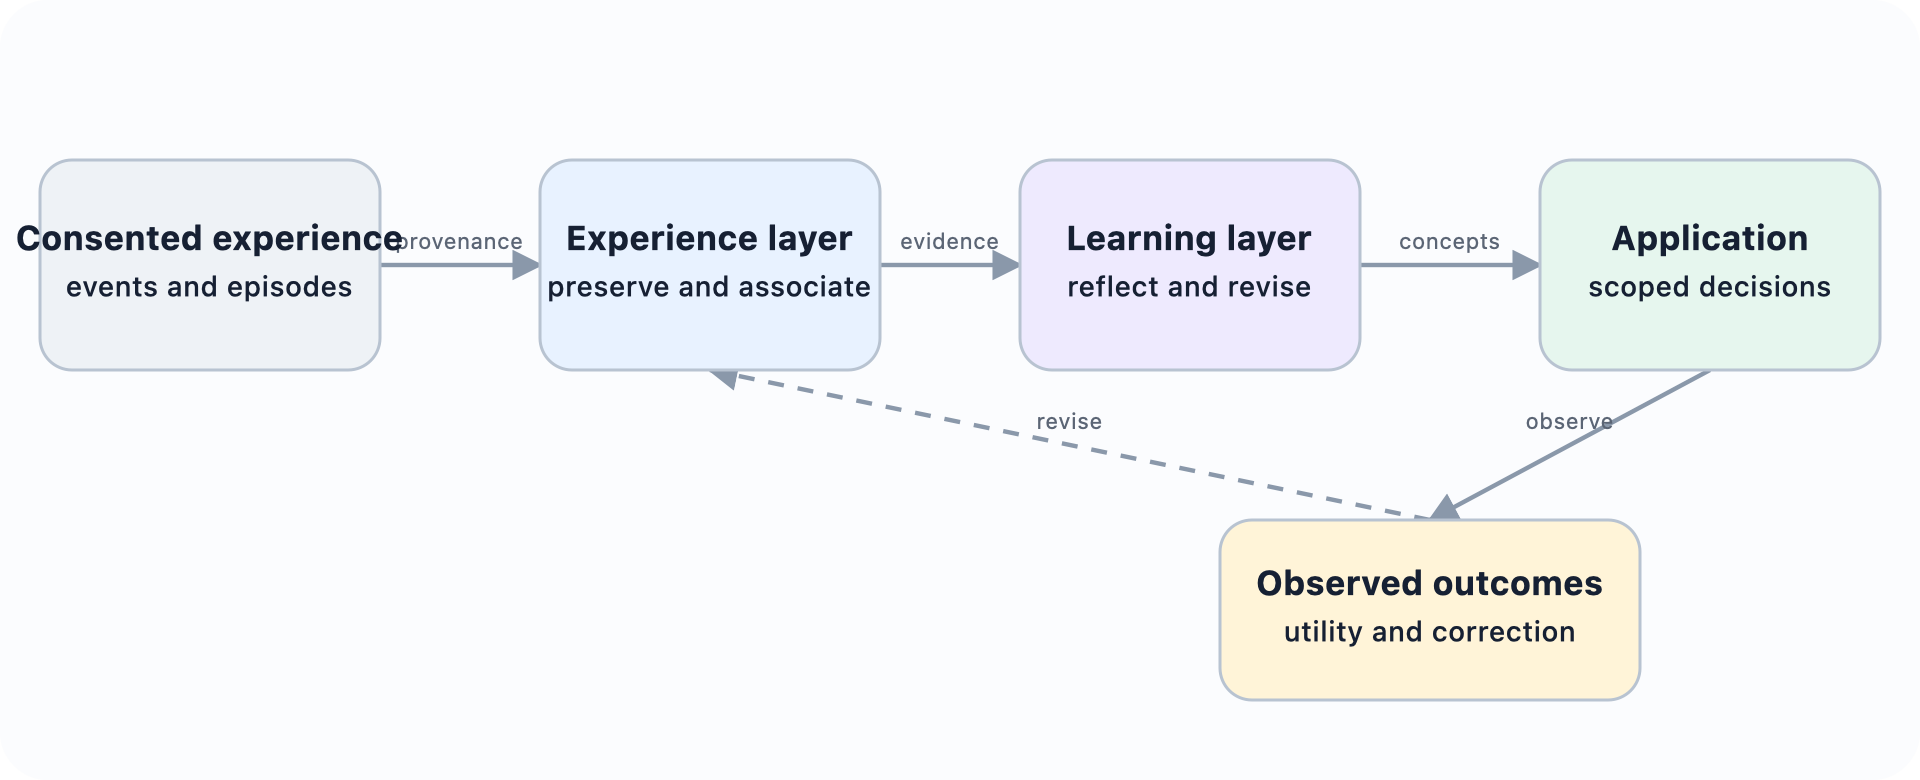
\includegraphics[keepaspectratio]{chapters/assets/diagrams/ell-overview.png}}

}

\caption{\textbf{Where the Experience Learning Layer sits.} ELL turns
consented experience into evidence-backed, revisable concepts, then uses
observed outcomes to improve or challenge them.}

\end{figure}%

ELL is organised as a
write--associate--reflect--consolidate--apply--evaluate loop. Each
component exposes a narrow interface so that models, stores, and
retrieval methods can be replaced independently.

The architecture separates three concerns. The input and capture layer
normalises consented chats, recordings, documents, tool traces, and
connectors into immutable sources, events, and episodes. Replaceable
memory and retrieval infrastructure stores or indexes projections for
association and candidate generation. The canonical learning layer
governs hypotheses, concepts, applications, outcomes, versioning,
permissions, and deletion.

External memory services and indexes can propose candidates, but they do
not define canonical truth, identity, policy, or learning state.

\section{ELL-Core and deferred
extensions}\label{ell-core-and-deferred-extensions}

The confirmatory system is deliberately small. ELL-Core contains seven
durable objects: \texttt{SourceArtifact}, \texttt{Episode},
\texttt{Reflection}, \texttt{ConceptVersion}, \texttt{EvidenceLink},
\texttt{ApplicationReceipt}, and \texttt{Outcome}. \texttt{AuditEvent}
records lifecycle operations. Associations may be computed ephemerally
or stored as disposable projections. Skills, graphs, learned
memory-operation policies, provider-specific memory objects, neural
state, multimodal capture, and product clients are deferred extensions.

This boundary is methodological, not only architectural. If a concept
layer cannot beat simple retrieval and direct-insight baselines with
this minimum object set, adding a graph database, learned controller, or
specialised vector index would make attribution harder rather than
rescue the claim.

\section{Canonical episode store}\label{canonical-episode-store}

The input is a canonical episode rather than an application-specific
chat message. An episode is represented as
e\_i=(id\_i,t\_event\_i,t\_observed\_i,x\_i,o\_i,a\_i,y\_i,s\_i,p\_i),
where id\_i is the episode identifier, t\_event\_i and t\_observed\_i
are event and observation time, x\_i is context, o\_i is an observation,
a\_i is an action, yi is an outcome, si is source metadata, and pi
contains privacy and access-control metadata. The two timestamps allow
delayed reports and later corrections to be represented.

The raw episode store is append-only. Corrections create new records
linked by relations such as corrects, supersedes, or retracts. This
preserves an audit trail and prevents an abstraction process from
silently rewriting its own evidence.

\section{Association layer}\label{association-layer}

The optional association layer creates typed links between episodes.
Initial relation types are:

\begin{itemize}
\tightlist
\item
  semantic similarity;
\item
  shared entities or participants;
\item
  temporal proximity or sequence;
\item
  shared goal or task;
\item
  shared action pattern;
\item
  similar outcome;
\item
  candidate causal relation;
\item
  contradiction or correction.
\end{itemize}

Only some edges are objective. Temporal sequence and shared identifiers
can be deterministic; causal and contradiction edges may be
model-generated hypotheses. Every edge therefore records its method,
score, model or rule version, and source evidence.

The layer supports both local neighbourhood retrieval and clustering.
Reflection should not operate only on the nearest embeddings because
lexically distant episodes may share a goal, failure pattern, or
outcome. Hybrid candidate generation combines semantic, structural,
temporal, and outcome-based signals. The first benchmark also includes
lexical-only, vector-only, and deterministic gold-cluster conditions so
the value of association is measured rather than presumed.

\section{Reflection Engine}\label{reflection-engine}

A reflection is a provisional interpretation:
r\_j=(h\_j,t\_j,s\_j,p\_j,n\_j,u\_j,z\_j).

Here hj is a claim or question, tj is reflection type, sj is scope, pj
and nj are supporting and counterevidence episode sets, uj is
uncertainty metadata, and zj is review status.

Reflection types include:

\begin{itemize}
\tightlist
\item
  observation or recurring pattern;
\item
  causal hypothesis;
\item
  strategy or procedural lesson;
\item
  preference hypothesis;
\item
  anomaly or exception;
\item
  unresolved question;
\item
  candidate correction to an existing concept.
\end{itemize}

The Reflection Engine is triggered by configurable events: a cluster
reaching a minimum size, a repeated failure, a surprising outcome, new
contradiction, elapsed time, or an explicit request. It produces
structured output and is followed by an evidence-validation pass.
Reflections may remain unverified, be marked supported, or be rejected
before they reach the Concept Engine.

\section{Concept Engine}\label{concept-engine}

A concept is a reusable, versioned proposition or strategy:
c\_k\^{}(v)=(q\_k,s\_k,a\_k,i\_k,p\_k,n\_k,g\_k,t\_k,v,z\_k).

Here qk is the proposition, sk is scope, ak is a set of applicability
conditions, ik is the expected implication or recommended behaviour, pk
and nk are supporting and counterevidence sets, gk is confidence, tk is
temporal validity, v is version, and zk is lifecycle state.

Concept types include descriptive patterns, user preferences, causal
hypotheses, strategies, constraints, and procedural rules. An initial
implementation should focus on textual concepts, but the schema permits
executable procedures or references to code artefacts.

The Concept Engine performs five operations:

\begin{enumerate}
\def\labelenumi{\arabic{enumi}.}
\tightlist
\item
  Propose: create a candidate concept from compatible reflections.
\item
  Merge: combine concepts that express the same claim and scope.
\item
  Split: separate an over-broad concept when evidence supports distinct
  conditions.
\item
  Revise: create a new version with changed claim, scope, validity, or
  confidence.
\item
  Retire or supersede: stop active use while preserving lineage.
\end{enumerate}

Promotion requires evidence from more than one episode unless a
domain-specific policy explicitly permits single-source facts. Evidence
diversity is measured across time, source, participant, task, and
surface form to reduce duplicate episodes being mistaken for independent
support.

\section{Concept registry and evidence
ledger}\label{concept-registry-and-evidence-ledger}

The concept registry contains the current active version of each concept
and its full version chain. The evidence ledger is append-only and
records:

\begin{itemize}
\tightlist
\item
  which episodes supported or contradicted a reflection;
\item
  which reflections contributed to a concept version;
\item
  which model, prompt, rule, or human action produced a change;
\item
  which concepts were retrieved for a decision;
\item
  what action was taken and what outcome followed;
\item
  deletions, access changes, and invalidations.
\end{itemize}

This ledger supports explanation and reproducibility. A user or
evaluator should be able to ask: ``Why does the system believe this?'',
``What evidence disagrees?'', ``When did this change?'', and ``Did using
it help?''

\section{Learning retrieval and
application}\label{learning-retrieval-and-application}

At decision time, the retrieval service selects a mixture of concepts
and source episodes. Concepts provide compact general guidance; episodes
provide specificity, exception handling, and verification. The retrieval
policy must be able to return either type independently.

A concept relevance score can initially be expressed as R(c,q)=w1 S1+w2
S2+w3 S3+w4 S4+w5 confidence(c)-w6 S6, where S1 through S4 represent
semantic relevance, scope match, temporal validity, and observed
utility; confidence(c) is concept confidence; and S6 is active
contradiction. This formula is a design heuristic, not a validated
scientific result. Weights will be tuned only on development data and
frozen before test evaluation.

The retrieved package includes the concept statement, scope, confidence,
current state, relevant support, relevant counterevidence, and source
links. At the application boundary this compact, budgeted package is
called an intuition packet. It may combine current concepts, selected
episodes, procedures, open commitments, uncertainty, and known
contradictions. It is a read object, not a new kind of memory.
Applications can require a minimum confidence or allow contested
concepts to be shown as uncertainty rather than instructions.

Formally, an intuition packet for query q, time t, policy context p, and
budget b is I(q,t,p,b)=(C\emph{,E},A\emph{,U},X\emph{,L}), where C* is
the selected set of current concepts or hypotheses, E* is the minimum
restored source evidence, A* contains applicable procedures or
prospective commitments, U* is calibrated uncertainty, X* is material
counterevidence or conflict, and L* is provenance and selection lineage.
The packet is valid only if every item satisfies p, its estimated
context cost does not exceed b, and its lineage resolves to permitted
canonical records.

\section{Outcome loop}\label{outcome-loop}

Every use of a concept creates an application record: am=(
xm,Cm,Em,dm,ym,um) .

Here xm is the task context, Cm and Em are the concepts and episodes
used, dm is the decision, ym is the observed outcome, and um is utility.
Outcome feedback can come from task reward, user correction, validator
output, or later observed consequences. The system must not
automatically treat every positive result as proof of causality;
outcomes are recorded as validation signals with their own reliability.
Repeated success can strengthen a concept, while failure can add
counterevidence, narrow scope, or trigger revision.

\section{Lifecycle}\label{lifecycle}

\begin{figure}[H]

{\centering \pandocbounded{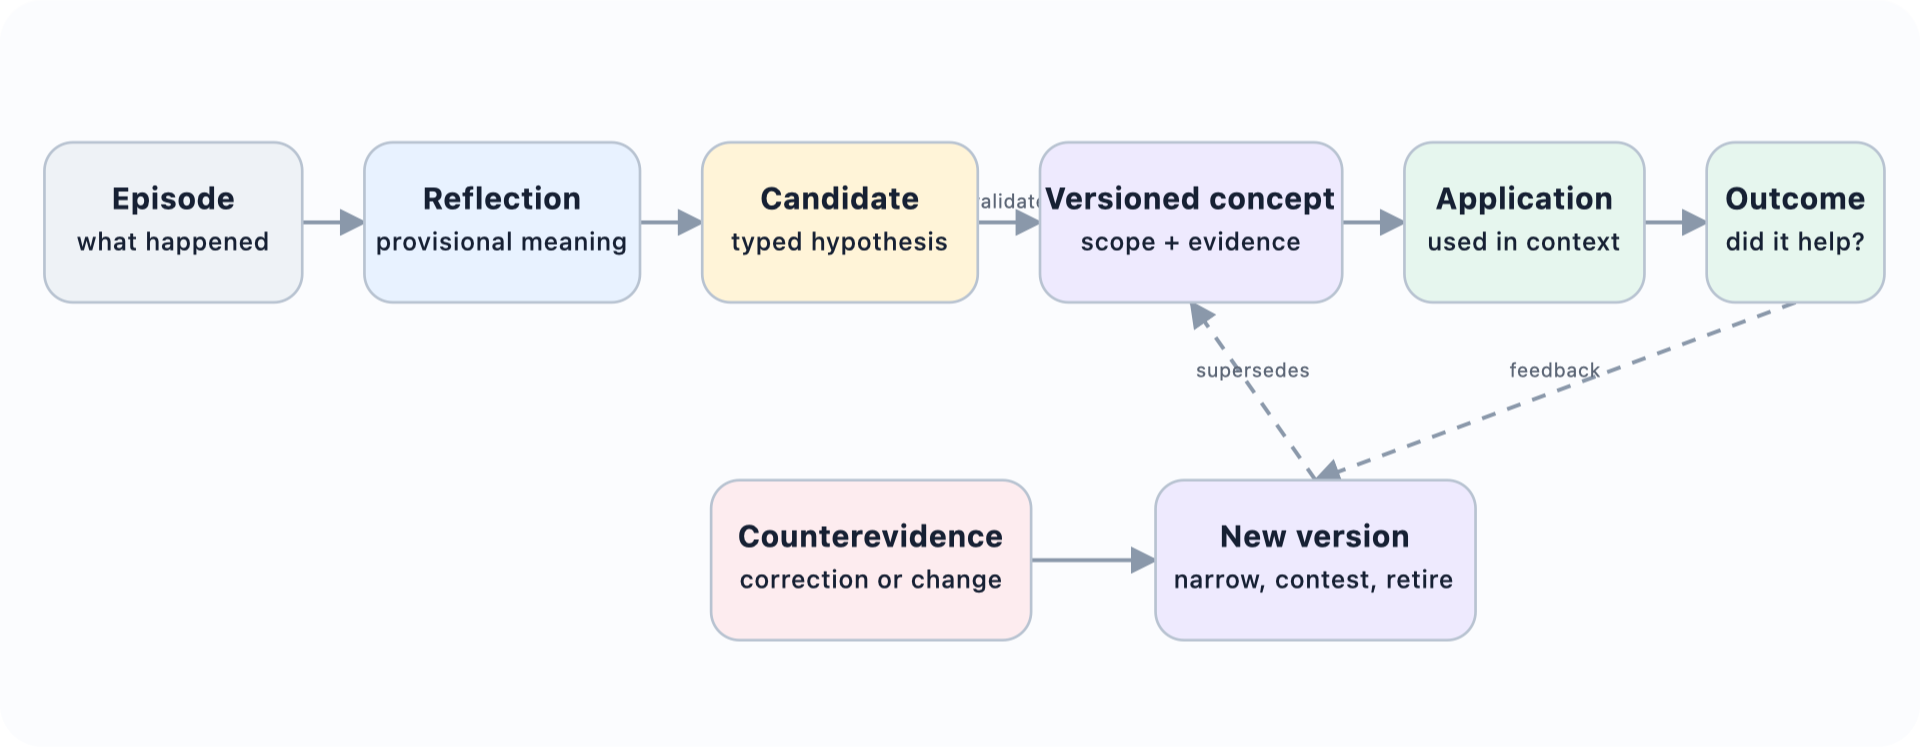
\includegraphics[keepaspectratio]{chapters/assets/diagrams/learning-lifecycle.png}}

}

\caption{\textbf{From one episode to a revisable concept.}
Interpretation remains provisional until evidence, scope, policy, and
counterevidence support promotion into a versioned concept.}

\end{figure}%

The lifecycle is intentionally reversible. Corroborated does not mean
permanently true. Contested concepts may still be retrieved when their
uncertainty is relevant. Superseded concepts remain available for
historical questions, while retired concepts are excluded from ordinary
guidance.

\bookmarksetup{startatroot}

\chapter{Proposed Algorithms}\label{proposed-algorithms}

\section{Minimum algorithm and comparison
discipline}\label{minimum-algorithm-and-comparison-discipline}

The first implementation favours transparent rules over an optimised
end-to-end pipeline. Each stage must expose its candidate inputs,
accepted outputs, rejected outputs, cost, and reason code. A more
complex policy is added only after the simpler condition has a frozen
baseline result. This ordering separates the value of the concept
contract from the value of a particular embedding model, graph,
reranker, or learned controller.

\section{Reflection scheduling}\label{reflection-scheduling}

Running reflection after every episode would be expensive and may create
redundant interpretations. ELL therefore uses event-based scheduling. An
episode or cluster enters the reflection queue when one or more
conditions are met:

\begin{itemize}
\item
  the cluster contains at least n distinct episodes;
\item
  a failure or unusually high reward occurs;
\item
  a new episode contradicts an active concept;
\item
  association novelty exceeds a threshold;
\item
  the concept has not been reviewed within a time window;
\item
  a user or agent explicitly requests reflection.
\end{itemize}

The scheduler records why a job was triggered. This enables later
analysis of whether a scheduling policy created useful concepts or
unnecessary model calls.

\section{Reflection generation and
critique}\label{reflection-generation-and-critique}

The Reflection Engine receives a bounded evidence packet: selected
episodes, existing nearby reflections, relevant active concepts, and an
instruction to produce typed hypotheses. The generator must output
structured fields rather than a free-form essay.

A separate validation pass performs four checks: 1. Entailment: Does
each cited episode actually support the claim attributed to it?

\begin{enumerate}
\def\labelenumi{\arabic{enumi}.}
\setcounter{enumi}{1}
\item
  Contradiction: Are there nearby episodes that disagree?
\item
  Scope: Is the claim broader than its evidence?
\item
  Novelty: Is the reflection meaningfully different from existing
  reflections or concepts?
\end{enumerate}

The validator can be an independent model, a deterministic rule, a human
reviewer, or a combination. Using a separate model call does not
guarantee independence, so experiments will include same-model and
cross-model validation conditions.

\section{Concept proposal}\label{concept-proposal}

Reflections are grouped by semantic compatibility and scope overlap. A
proposed concept requires:

\begin{itemize}
\tightlist
\item
  at least m compatible reflections;
\item
  at least d distinct supporting episodes;
\item
  minimum evidence diversity;
\item
  no unresolved high-confidence contradiction;
\item
  an explicit scope and exception list;
\item
  a concise proposition and expected implication.
\end{itemize}

The initial development policy will require support from at least three
episodes across at least two distinct contexts. The threshold is not a
claim about how many observations create knowledge. It is a
preregistered control variable, swept only on development streams and
frozen before the sealed test.

A simplified proposal procedure is: for each reflection cluster R:
evidence = union(supporting episodes in R) counter = retrieve plausible
counterevidence candidate = generate\_concept(R, evidence, counter)
checks = validate(candidate, evidence, counter) if checks pass promotion
policy: register(candidate, state=``proposed'')

\section{Evidence-weighted
confidence}\label{evidence-weighted-confidence}

LLMs are not assumed to be calibrated judges of their own abstractions.
ELL computes an operational confidence score from external features:

confidence(c)=1/(1+exp(-z\_c)) , where zc is a weighted score that
increases with supporting evidence, evidence diversity, and observed
application utility, and decreases with counterevidence, age without
revalidation, and validator disagreement.

The formula is deliberately transparent and will be calibrated on
held-out development data. A fixed rule based on support, contradiction,
and outcome counts is the mandatory baseline; logistic and Bayesian
alternatives are secondary conditions. Confidence is never used to hide
counterevidence, and it is not interpreted as a probability until
calibration supports that interpretation. The raw counts and links
remain visible.

\section{Revision and temporal
validity}\label{revision-and-temporal-validity}

When new evidence conflicts with a concept, the system chooses among
four responses:

\begin{itemize}
\tightlist
\item
  add exception: the core claim remains valid but has a narrower
  boundary;
\item
  narrow scope: the concept was over-generalised;
\item
  change validity interval: the pattern was true during one period but
  is no longer current;
\item
  replace claim: a new concept version better explains the evidence.
\end{itemize}

Revision produces a new immutable version linked by revises or
supersedes. The old version retains its former validity interval and
applications. This design supports historical reasoning and avoids
treating changed preferences or conditions as contradictions that must
erase the past.

\section{Merge and split}\label{merge-and-split}

Duplicate concepts increase retrieval noise, while over-broad concepts
hide meaningful exceptions. Merge candidates are identified using
proposition similarity, overlapping evidence, compatible scope, and
similar implications. Split candidates are triggered when
counterevidence clusters around a coherent condition or when application
outcomes differ significantly by context.

Both operations require a lineage record. A merge creates a new concept
that references all parents. A split creates child concepts whose
evidence partitions are explicit. Automated operations above a risk
threshold can require human approval.

\section{Retrieval with evidence
restoration}\label{retrieval-with-evidence-restoration}

Concept retrieval follows two stages. The first stage selects concepts
by semantic, structural, temporal, and utility signals. The second
restores a small, query-specific set of source episodes. This prevents a
compact concept from becoming an ungrounded instruction.

The retrieval budget is fixed in tokens or characters so that systems
are compared under equal context cost.

This avoids rewarding a method merely for retrieving far more text.
Results report both task utility and memory information density.

\section{Deletion and invalidation}\label{deletion-and-invalidation}

A user must be able to delete source data. Deletion cannot stop at the
episode store because derived concepts may still encode the removed
information. ELL maintains derivation links so a deletion request can:

\begin{enumerate}
\def\labelenumi{\arabic{enumi}.}
\tightlist
\item
  remove or tombstone the source episode according to policy;
\item
  remove it from support and counterevidence sets;
\item
  recompute affected confidence values;
\item
  contest, revise, or retire concepts that no longer meet support
  thresholds;
\item
  record the deletion cascade without retaining prohibited content.
\end{enumerate}

This is both a privacy requirement and a scientific requirement:
provenance is incomplete if derived claims cannot be invalidated when
their evidence disappears.

\bookmarksetup{startatroot}

\chapter{Data Model and Public
Interfaces}\label{data-model-and-public-interfaces}

\begin{figure}[H]

{\centering \pandocbounded{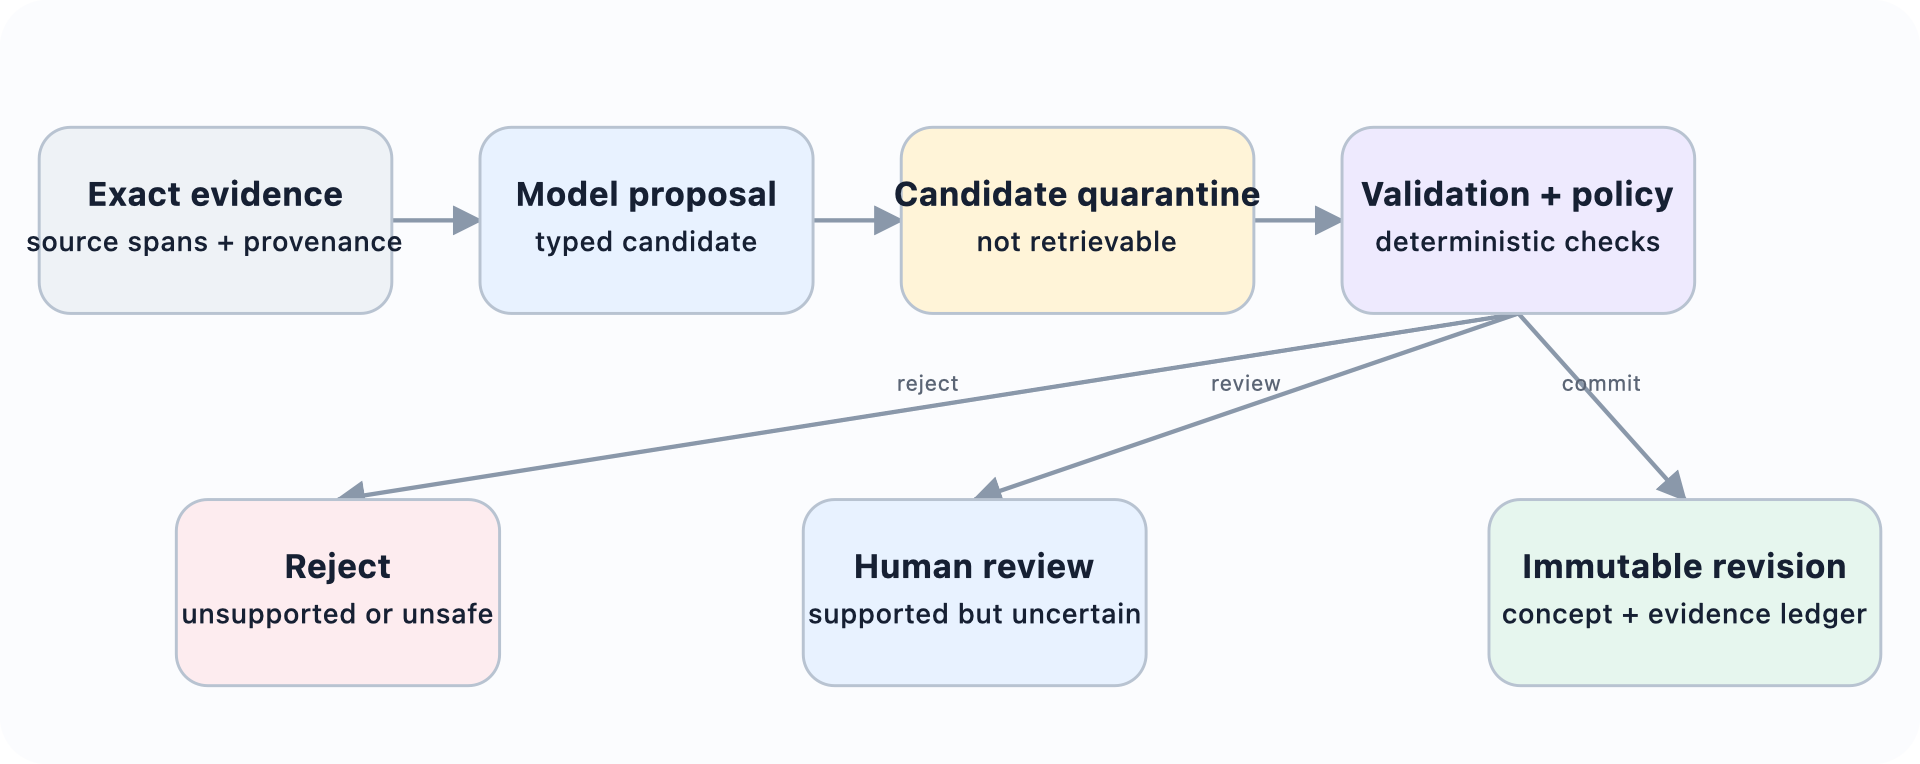
\includegraphics[keepaspectratio]{chapters/assets/diagrams/governed-commit.png}}

}

\caption{\textbf{Models interpret; deterministic code governs.}
Generated interpretations enter quarantine. Schema validation and
deterministic policy decide whether they are rejected, reviewed, or
committed.}

\end{figure}%

\section{Core entities}\label{core-entities}

{\def\LTcaptype{none} % do not increment counter
\begin{longtable}[]{@{}
  >{\raggedright\arraybackslash}p{(\linewidth - 4\tabcolsep) * \real{0.3333}}
  >{\raggedright\arraybackslash}p{(\linewidth - 4\tabcolsep) * \real{0.3333}}
  >{\raggedright\arraybackslash}p{(\linewidth - 4\tabcolsep) * \real{0.3333}}@{}}
\toprule\noalign{}
\begin{minipage}[b]{\linewidth}\raggedright
Entity
\end{minipage} & \begin{minipage}[b]{\linewidth}\raggedright
Purpose
\end{minipage} & \begin{minipage}[b]{\linewidth}\raggedright
Required fields
\end{minipage} \\
\midrule\noalign{}
\endhead
\bottomrule\noalign{}
\endlastfoot
\texttt{SourceArtifact} & Immutable addressable evidence & ID, content
hash, source type, stable spans, event and observed time, consent,
sensitivity, workspace \\
\texttt{Episode} & Bounded experience derived from one or more sources &
ID, context, observation, action, outcome, source spans, access
metadata \\
\texttt{Reflection} & Provisional interpretation or question &
statement, type, scope, support, counterevidence, uncertainty, review
status \\
\texttt{ConceptVersion} & Reusable versioned claim or strategy &
proposition, scope, conditions, implication, support, counterevidence,
confidence, validity, version, lifecycle state \\
\texttt{EvidenceLink} & Typed derivation or challenge relation & source
ID and span, target ID and version, relation, method, validator,
timestamp \\
\texttt{ApplicationReceipt} & Immutable record of a concept's use &
task, exact concept versions, restored evidence, decision, model, cost,
timestamp \\
\texttt{Outcome} & Independently sourced evidence about an application &
linked receipt, observation or reward, source, reliability, delay \\
\texttt{AuditEvent} & Content-minimised lifecycle record & actor,
operation, object, prior version, new version, method, timestamp \\
\end{longtable}
}

\texttt{Association} is an optional typed projection used for candidate
generation. \texttt{SkillVersion} and provider-specific memory assets
are deferred extension objects and are not required to test the primary
ELL-Core claim.

\section{Concept states}\label{concept-states}

\begin{itemize}
\tightlist
\item
  proposed: generated and valid enough to test, but not yet strongly
  supported;
\item
  corroborated: meets evidence and validation thresholds;
\item
  contested: important unresolved counterevidence exists;
\item
  revised: a new immutable version has been created in response to
  changed evidence and is awaiting or recording validation;
\item
  superseded: replaced by a newer or more precise concept;
\item
  retired: no longer eligible for ordinary retrieval;
\item
  deleted: content removed under deletion policy, with only
  non-sensitive structural audit metadata retained where legally
  permitted.
\end{itemize}

A revision never overwrites its parent. A revised version can later
become corroborated, contested, superseded, retired, or deleted while
its lineage remains traceable.

\section{API contract}\label{api-contract}

A reference implementation should expose the following model-independent
minimum operations:

\begin{Shaded}
\begin{Highlighting}[]
\NormalTok{record\_source(source) {-}\textgreater{} SourceID}
\NormalTok{record\_episode(episode) {-}\textgreater{} EpisodeID}
\NormalTok{propose\_reflections(scope, trigger) {-}\textgreater{} list[Reflection]}
\NormalTok{reconcile\_concepts(reflection\_ids) {-}\textgreater{} list[ConceptVersion]}
\NormalTok{retrieve\_learning(query, context, budget) {-}\textgreater{} LearningPacket}
\NormalTok{record\_application(packet, decision) {-}\textgreater{} ApplicationID}
\NormalTok{record\_outcome(application\_id, outcome) {-}\textgreater{} list[ConceptUpdate]}
\NormalTok{explain\_concept(concept\_id, version=None) {-}\textgreater{} EvidenceReport}
\NormalTok{invalidate\_source(source\_id, policy) {-}\textgreater{} InvalidationReport}
\end{Highlighting}
\end{Shaded}

Association, skill proposal, graph traversal, provider import, and
learned-policy APIs are optional ports layered around this contract.

LearningPacket is the central read object. It contains concepts,
relevant evidence, conflicts, and budget accounting. It never contains
only a naked concept statement.

\section{Storage independence}\label{storage-independence}

The core schema is storage-neutral. A starter implementation uses an
in-memory store and deterministic scan before adding SQLite and
full-text search as the first persistent baseline. Exact vector search
is evaluated before approximate indexes. Production adapters may later
add PostgreSQL, TurboVec or another vector index, a graph database, or a
hosted memory system. Storage choices are evaluated by correctness,
write cost, query latency, deletion support, reproducibility, and
operational simplicity rather than by architectural fashion.

The same principle applies to model providers. The engine depends on a
structured-generation interface, not a vendor SDK. Reproducibility
experiments use open-weight models, while optional adapters may support
hosted models for comparison.

Association, extraction, consolidation, retrieval, and forgetting
policies may become configurable or learned, but their outputs remain
proposals behind stable typed ports. Deterministic code continues to
enforce provenance, workspace isolation, permissions, deletion, schema
validity, and canonical commit rules. Competing lexical, vector, graph,
temporal, probabilistic, and model-driven policies remain
interchangeable experimental conditions until evaluation establishes
which combination is useful. A Zettelkasten-style linked-note
representation may be included as a simple baseline, but static note
linking is too limited to govern temporal change, uncertainty,
counterevidence, outcome feedback, and user control.

\bookmarksetup{startatroot}

\chapter{Experimental Design}\label{experimental-design}

\section{Study status}\label{study-status}

The evaluation is preregistered in this paper before results are
collected. All thresholds, prompts, model versions, random seeds,
exclusions, and statistical tests will be committed before the sealed
test sets are run.

Any later changes will be reported as deviations rather than silently
folded into the method.

\section{Evaluation stages}\label{evaluation-stages}

\subsection{Stage A: controlled latent-pattern
streams}\label{stage-a-controlled-latent-pattern-streams}

The project will release a synthetic benchmark in which each experience
stream is generated from known latent concepts. A stream contains:

\begin{itemize}
\tightlist
\item
  recurring contextual rules;
\item
  paraphrased surface forms;
\item
  irrelevant but semantically similar episodes;
\item
  exceptions with explicit conditions;
\item
  contradictory observations;
\item
  temporal change points;
\item
  delayed outcomes;
\item
  duplicated or correlated evidence.
\end{itemize}

Example latent concept: When a task depends on another team and the
owner is not involved before commitment, delivery risk increases; the
pattern does not apply to independently executable tasks.

The generator creates episodes that support, contradict, or fall outside
the concept's scope. The benchmark therefore has gold labels for the
concept, its conditions, its evidence, counterevidence, and validity
interval.

Three stream lengths are planned: 50, 200, and 1,000 episodes.
Difficulty increases through noise, lexical distance, exceptions, and
concept drift. A sealed test generator seed prevents manual prompt
tuning against the exact cases.

\subsection{Stage B: long-term conversational
memory}\label{stage-b-long-term-conversational-memory}

LongMemEval and LoCoMo will test whether ELL remains competitive on
factual extraction, cross-session reasoning, temporal reasoning,
updates, abstention, and long-range dialogue understanding (Wu et
al.~2025;

Maharana et al.~2024). MemBench will add reflective-memory and
efficiency measures where licensing and harness compatibility permit (H.
Tan et al.~2025). MemoryAgentBench will test retrieval, test-time
learning, long-range understanding, and selective forgetting in
incremental multi-turn interaction (Hu, Wang, and McAuley 2025).

LoCoMo-Plus adds cue--trigger semantic disconnect, where a later prompt
must activate an earlier latent constraint despite low lexical
similarity (Li et al.~2026). It is the preferred external test for the
structurally distant retrieval aspect of the ELL claim, although it does
not provide gold concept lifecycles.

ELL is not expected to dominate span-recall tasks solely because it
forms concepts. These benchmarks test whether the abstraction layer
preserves ordinary memory performance and whether concept retrieval
helps multi-session inference.

\subsection{Stage C: memory-dependent
action}\label{stage-c-memory-dependent-action}

MemoryArena will test whether information learned in earlier sessions
improves later task execution (He et al.

2026). Mem2ActBench tests whether established preferences and task state
are applied to tool selection and parameters rather than only restated
in an answer (Shen et al.~2026). A smaller deterministic environment
will be used for rapid development, while these external benchmarks test
whether a result survives outside the synthetic generator.

\subsection{Stage D: ELL intuition and outcome
benchmark}\label{stage-d-ell-intuition-and-outcome-benchmark}

The ELL-specific benchmark combines controlled organisational and
personal-work streams with later tasks that require conversational
shorthand, proactive but non-intrusive context, structurally distant
transfer, adaptation at known change points, and explicit correction.
Each decision records an ApplicationReceipt and an independently scored
outcome. Gold data identifies required context, irrelevant private
context, support, counterevidence, validity intervals, and deletion
cascades. The benchmark therefore measures not only whether information
was recalled, but whether a compact intuition packet selected the right
evidence, improved behaviour, remained calibrated, and changed or forgot
appropriately.

\section{Memory Dynamics and Intuition Simulation
Lab}\label{memory-dynamics-and-intuition-simulation-lab}

The evaluation will include a reproducible simulation laboratory for
studying memory dynamics before any policy is considered for deployment.
The laboratory replays deterministic, timestamped scenario streams
through the same typed ports used by the reference architecture. It
supports parameter sweeps and side-by-side policy comparisons for
extraction, association, consolidation, retrieval, revision, and
forgetting without granting an experimental policy authority to mutate
canonical evidence. Each run fixes the scenario version, configuration,
model and prompt identifiers, random seed, permissions, and resource
budget. It emits immutable decision and ApplicationReceipts that resolve
every selected context item, candidate mutation, committed version,
action, outcome, evaluator judgement, and cost to its permitted source
evidence.

Scenarios use synthetic or appropriately de-identified longitudinal
personas representing both individuals and organisations. They include
stable preferences, weak signals, sensitive attributes that must not be
inferred or revealed, explicit consent changes, contradictions, temporal
drift, delayed outcomes, workspace boundaries, and deletion requests.
Chronological train, development, and sealed test intervals prevent
policies from learning from future events; change points and deletion
events remain hidden from the system until they occur in replay. The
laboratory compares no memory, raw-history or maximum-context prompting,
ordinary retrieval, direct insight extraction, and ELL-Core ablations
under matched sources, model conditions, context budgets, and outcome
opportunities.

Preregistered primary measures cover retrieval precision and recall;
faithfulness and calibration of claims; adaptation latency after change
or correction; contradiction and stale-memory rates; transfer and
downstream task utility; overpersonalisation and unjustified inference;
privacy, consent, and cross-workspace leakage; deletion-cascade
completeness; and latency, token, storage, and energy or hardware-time
cost, including consolidation.

Scoring is deterministic wherever gold state and event traces permit.
Outcome and safety judgements are produced by evaluators independent of
the policy under test; subjective conversational naturalness is assessed
separately by blinded human reviewers. Stochastic conditions use
multiple preregistered seeds and report confidence intervals and effect
sizes. This laboratory is an evaluation proposal, not evidence that the
present implementation already provides adaptive intuition or safe
learned memory operations.

\section{Baselines}\label{baselines}

At minimum, all experiments include:

\begin{enumerate}
\def\labelenumi{\arabic{enumi}.}
\tightlist
\item
  no persistent memory;
\item
  full or maximum available context;
\item
  BM25 retrieval over raw episodes;
\item
  exact vector retrieval over raw episodes;
\item
  fixed BM25--vector fusion over raw episodes;
\item
  rolling summary memory;
\item
  episode retrieval plus direct insight extraction;
\item
  ELL-Core without concept consolidation;
\item
  full ELL-Core with evidence-restored learning packets.
\end{enumerate}

The strongest of conditions 3--7 is selected on development data before
the sealed run and becomes the confirmatory comparator. This prevents a
weak hand-picked baseline from making ELL look effective.

Where reproducible implementations and compatible licences are
available, Hindsight, A-MEM, and Reflective Memory Management form the
first named comparison tier because they are close to ELL's reflection
and structured-memory claim (Latimer et al.~2026; Xu et al.~2025; Z. Tan
et al.~2025). GAAMA and PlugMem may be added if their key behaviour can
be reproduced (Paul, Sharma, and Sareen 2026; Yang et al.~2026). A
method will not be included under another system's name when critical
behaviour is missing or reimplemented only approximately.

Separate substrate experiments compare Letta/MemGPT, Mem0, Graphiti/Zep,
Hindsight, and TencentDB Agent Memory as context or memory providers.
Retrieval-only experiments compare deterministic scan, BM25, exact
vectors, HNSW, and TurboVec. Learned operation, experience-graph,
skill-evolution, and neural or parametric memory systems are deferred
exploratory tracks; they do not enter the first confirmatory comparison.

\section{Matching and accounting
protocol}\label{matching-and-accounting-protocol}

Every eligible condition receives the same chronological source stream,
answer model, answer-generation settings, task opportunities, and
maximum answer budget. Retrieval context is capped by the same token
budget. Systems may use their native write and retrieval prompts, but
every prompt, model call, intermediate artefact, retry, cache policy,
and background job is recorded.

Two cost views are reported. Read-path cost measures the user-visible
decision. Amortised end-to-end cost includes ingestion, embeddings,
extraction, graph or index maintenance, reflection, validation,
consolidation, retrieval, and generation over the complete stream. A
system is not credited with efficiency by moving work into an unreported
background process.

The answer model is prevented from seeing system labels. Where possible,
retrieved packets are normalised into a common envelope containing
content, timestamps, provenance references, and system-supplied scores.
The sealed test is run once per frozen configuration. Failed runs,
exclusions, and provider errors remain in the released trace.

\section{Model conditions}\label{model-conditions}

The main reproducibility track uses at least two openly licensed
instruction-tuned models from different model families and two capacity
bands. Model names are recorded only when the experiment is frozen,
because available open models change rapidly. All generation settings,
quantisation, serving software, prompts, and hardware are logged.

A hosted-model comparison may be reported separately, but the paper's
core claims must remain reproducible without proprietary APIs.

\section{Metrics}\label{metrics}

Downstream metrics

\begin{itemize}
\tightlist
\item
  task success or benchmark accuracy;
\item
  answer faithfulness to retrieved evidence;
\item
  transfer gain over the episode-only baseline;
\item
  abstention quality;
\item
  action efficiency, including steps to completion.
\end{itemize}

Concept metrics Concept correctness. Does the induced proposition match
the gold latent pattern or human judgement?

Evidence precision. What proportion of cited support actually supports
the concept?

Evidence recall. What proportion of relevant support was linked?

Counterevidence recall. Did the system find important exceptions and
contradictions?

Scope accuracy. Does the concept apply to the right contexts without
over-generalising?

Revision latency. How many contradictory episodes or how much time
elapses before a stale concept is contested or revised?

Lineage correctness. Do revisions, merges, and splits preserve accurate
parent and evidence links?

Calibration. Does stated confidence correspond to observed concept
correctness and application success?

Brier score and expected calibration error will be reported.

Efficiency metrics

\begin{itemize}
\tightlist
\item
  input and output tokens per episode and per decision;
\item
  model calls per accepted concept;
\item
  storage growth;
\item
  median and tail latency;
\item
  energy or hardware-time proxy where measurable;
\item
  task utility per 1,000 retrieved tokens.
\end{itemize}

Product-facing secondary criteria

\begin{itemize}
\tightlist
\item
  shorthand resolution accuracy without requiring the user to restate
  stable context;
\item
  precision and recall of proactive just-in-time context, including a
  penalty for intrusive or irrelevant retrieval;
\item
  useful generalisation to structurally related but lexically dissimilar
  situations;
\item
  change-detection delay and correction latency after explicit or
  behavioural counterevidence;
\item
  calibration and selective abstention when evidence is weak, stale, or
  contradictory;
\item
  explanation faithfulness, citation validity, and user ability to
  correct, scope, or delete the underlying memory;
\item
  end-to-end task utility per token, latency, storage, model call, and
  energy or hardware-time proxy, including background consolidation
  cost;
\item
  zero cross-workspace leakage and complete tested invalidation of
  deleted evidence from derived projections.
\end{itemize}

These product-facing measures cannot establish the primary claim. The
preregistered decision gates in Section 11 determine whether ELL-Core is
supported, partially supported, or rejected before a production memory
substrate or learned policy is chosen.

An implementation is not successful merely because it stores more,
produces persuasive summaries, or retrieves plausible context.

\section{Human evaluation}\label{human-evaluation}

Concept quality cannot be reduced entirely to lexical matching. A
stratified sample will be rated by at least three annotators who are
blind to the system condition. The rubric covers correctness, support,
scope, usefulness, and whether counterevidence was handled
appropriately. Inter-rater agreement is reported using Krippendorff's
alpha. Disagreements are retained rather than resolved solely by an LLM
judge.

LLM-based judges may scale evaluation, but they will be calibrated
against the human sample. Prompts and raw judgements will be released.
The same model used to generate a concept will not be the only judge of
that concept.

\section{Ablations}\label{ablations}

The following components are removed one at a time:

\begin{itemize}
\tightlist
\item
  reflection--concept separation;
\item
  counterevidence retrieval;
\item
  evidence diversity threshold;
\item
  temporal validity;
\item
  lifecycle versioning;
\item
  application-outcome feedback;
\item
  source-episode restoration at retrieval;
\item
  graph associations beyond vector similarity.
\end{itemize}

Additional sweeps vary reflection frequency, promotion thresholds,
retrieval budget, and confidence formulation. Architecture ablations
compare lexical, vector, graph, temporal, and hybrid association; fixed
versus learned extraction and consolidation policy; concept-only versus
episode-restored packets; and eager versus event-triggered background
processing. This keeps dynamic graph organisation, probabilistic
hypotheses, and other research directions behind evidence gates instead
of presuming a settled winner.

Safety ablations separately disable deterministic validation around
learned write, update, and discard proposals; independent outcome
validation around skill evolution; and canonical evidence restoration
around neural or parametric adaptation. These conditions are diagnostic
and are not deployment configurations.

\section{Statistical analysis}\label{statistical-analysis}

The primary binary task outcome uses a paired absolute difference with a
paired bootstrap 95\% confidence interval; McNemar's test is reported as
a sensitivity analysis where appropriate. Continuous or ordinal metrics
use paired bootstrap confidence intervals and report effect sizes.
Multiple random seeds are used for synthetic generation and stochastic
inference. The benchmark size is chosen before the sealed run to provide
at least 80\% power for the five-percentage-point minimum practically
important transfer effect defined in Section 11.

Results are reported by task category and stream length, not only as a
single average. Failure analysis separates write, association,
reflection, consolidation, retrieval, reasoning, and application errors.

\bookmarksetup{startatroot}

\chapter{Open-Source Research
Publication}\label{open-source-research-publication}

\section{Licensing}\label{licensing}

The repository is released under the permissive MIT License. It covers
the paper source, diagrams, documentation, publication tools, and
synthetic examples unless a file states otherwise. Third-party datasets
retain their original licences and are downloaded separately. A future
archival research release should additionally include machine-readable
citation metadata and generated dependency attribution.

\section{Repository structure}\label{repository-structure}

\begin{Shaded}
\begin{Highlighting}[]
\NormalTok{experience{-}learning{-}layer/}
\NormalTok{├── README.md}
\NormalTok{├── LICENSE}
\NormalTok{├── \_quarto.yml}
\NormalTok{├── styles.css}
\NormalTok{├── index.qmd}
\NormalTok{├── chapters/}
\NormalTok{│   └── assets/diagrams/}
\NormalTok{├── examples/}
\NormalTok{└── .github/workflows/publish.yml}
\end{Highlighting}
\end{Shaded}

The repository contains the living chapter sources, shared visual
diagrams, synthetic lifecycle examples, and the small Quarto
configuration required to produce the website and PDF. Generated output
is ignored and rebuilt locally or by GitHub Actions. The repository
deliberately excludes product code and an executable learning kernel so
that proposed architecture is not mistaken for validated implementation
evidence.

\section{Reproducibility
requirements}\label{reproducibility-requirements}

Every reported experiment must include:

\begin{itemize}
\tightlist
\item
  immutable configuration files;
\item
  exact Git commit;
\item
  model identifiers and hashes where available;
\item
  prompts and structured-output schemas;
\item
  random seeds;
\item
  hardware and serving configuration;
\item
  raw outputs and failure logs;
\item
  evaluation code and judge prompts;
\item
  token, latency, and storage accounting.
\end{itemize}

A one-command small-scale reproduction should run on consumer hardware
with a compact open model. Full benchmark results may require larger
hardware, but the same code path and data format must be used.

\section{Contribution model}\label{contribution-model}

The project begins with a lightweight maintainer model and records its
evolution through the manuscript and Git history. Contributions require
reproducible publication checks, provenance for example or benchmark
changes, and a declaration when generated data or code was produced with
model assistance.

Research claims are reviewed separately from software changes. A faster
implementation is not accepted as scientifically equivalent unless its
behaviour and evaluation remain comparable.

\section{Private data boundary}\label{private-data-boundary}

Private conversation exports can be used locally to test ingestion and
qualitative usefulness, but they are not part of the public benchmark
and must not be committed. Public experiments use synthetic or properly
licensed data. This paper includes data-governance guidance; redaction
hooks, local namespaces, and tested deletion cascades are required
before any longitudinal pilot.

\bookmarksetup{startatroot}

\chapter{Ethics, Privacy, and
Security}\label{ethics-privacy-and-security}

A memory system can improve continuity while also increasing risk.
Persistent concepts may encode sensitive information, amplify a mistaken
interpretation, or influence actions long after the originating
interaction.

Long-term memory is therefore a control channel, not merely a
convenience layer. Research on trustworthy memory search similarly shows
that semantically related memory can still be inappropriate or unsafe
for the current task (Zhang et al.~2026).

ELL adopts the following principles.

Visibility. Users should be able to inspect active concepts, evidence,
uncertainty, and change history.

Correction. A user correction is stored as high-priority evidence and
can trigger immediate contestation, but it should not silently erase
historical state when historical reasoning is required.

Deletion. Source deletion propagates to derived concepts. Derived
content must not survive simply because it was transformed.

Least access. Retrieval enforces source-level permissions and subject
namespaces before semantic relevance is considered.

No hidden certainty. Contested or weak concepts are labelled. Confidence
and evidence counts are not replaced by persuasive prose.

Poisoning resistance. New memories do not automatically become trusted
rules. Promotion requires independent evidence and validators, and
sensitive actions can require human approval.

Purpose limitation. Concepts formed for one domain are not automatically
reused in another. Cross-domain transfer is an explicit, auditable
operation.

The system may still infer sensitive traits that were never stated
directly. The research implementation therefore defaults to local
processing, excludes sensitive-trait inference from public examples, and
treats inferred personal concepts as user-governed data. Future work
must test whether users can understand and meaningfully control these
abstractions.

\bookmarksetup{startatroot}

\chapter{Limitations and Threats to
Validity}\label{limitations-and-threats-to-validity}

\section{Critical appraisal of the
approach}\label{critical-appraisal-of-the-approach}

The strongest criticism of ELL is that it may be an over-engineered
combination of ideas that already exist in agent memory, truth
maintenance, belief revision, temporal databases, and provenance
systems. Reflection, experience abstraction, confidence-bearing
opinions, temporal graphs, versioned skills, and evidence tracing all
have close precedents. A paper that presents their combination as
self-evidently better would be a systems manifesto rather than a
research contribution.

The second criticism is attribution. If the first implementation
simultaneously adds a graph, vector search, reflection, a concept
registry, learned policies, provider adapters, and outcome feedback, an
improvement cannot be assigned to the concept lifecycle. The same
complexity also creates many tuning degrees of freedom and a large risk
of test-set adaptation.

The third criticism is representational favouritism. A synthetic
generator with explicit latent concepts naturally rewards a system that
stores explicit concepts. Strong raw-retrieval or agent-controlled
memory may perform better in open environments where the useful
regularity is procedural, perceptual, or difficult to state. External
benchmarks and negative-transfer cases are therefore required.

The fourth criticism is causal. An application receipt shows that a
concept was present when an action was taken; it does not prove that the
concept caused the outcome. The answer model may ignore the packet, rely
on prior knowledge, or succeed for another reason. Factorial packet
ablations and randomised inclusion on eligible tasks are needed before
making causal utility claims.

These criticisms determine the implementation order: benchmark first,
simple baselines second, deterministic ELL-Core third, model-assisted
consolidation fourth, and optional infrastructure only after the primary
result. The first study has one confirmatory outcome and explicit stop
conditions. This discipline is part of the proposal, not an
implementation detail.

\section{Specific threats}\label{specific-threats}

First, textual concepts favour knowledge that can be expressed as
propositions or instructions. Tacit motor skills, perceptual expertise,
and distributed representations may not fit this format. ELL may
therefore complement rather than replace parametric or executable skill
learning.

Second, provenance does not guarantee truth. Episodes can be incorrect,
duplicated, biased, or malicious. A perfectly traceable concept may
still be grounded in poor evidence. Source reliability and adversarial
robustness require separate study.

Third, LLM-generated reflections may introduce causal stories that are
plausible but unsupported. The validation and counterevidence stages
reduce this risk but cannot eliminate it. Human evaluation remains
necessary for high-stakes domains.

Fourth, the proposed confidence formula is heuristic. Evidence counts
are not independent observations, and application outcomes may be
delayed or confounded. Calibration must be empirical and
domain-specific.

Fifth, synthetic benchmarks can overstate progress if their latent rules
resemble the system's representation.

The controlled benchmark is useful for diagnosis but must be paired with
natural conversations and agentic tasks.

Sixth, comparisons across memory systems are difficult because ingestion
granularity, retrieval budget, model backbone, prompts, and judge choice
can dominate results. The protocol therefore fixes budgets and reports
complete configurations, but residual implementation differences remain.

Seventh, the architecture adds cost and operational complexity. The
system is unsuccessful if the concept layer does not deliver enough
transfer, safety, or efficiency to justify reflection, validation,
storage, and governance overhead.

Eighth, the term intuition can encourage anthropomorphism or hide
uncertainty behind fluent behaviour. In this paper it is only an
operational label for measured context selection and adaptation. A
compact packet may also compress away rare but important exceptions, so
source restoration, counterevidence retrieval, and abstention must be
evaluated explicitly.

Ninth, reduced prompt tokens do not necessarily reduce total energy or
latency. Background embedding, association, graph maintenance,
reflection, and consolidation can move cost out of the visible request
path.

Efficiency claims therefore require end-to-end accounting over both
write-time and read-time work.

Tenth, learned memory operations introduce reward misspecification and
policy-opacity risks. A policy may improve benchmark reward by
discarding inconvenient counterevidence, overfitting retrieval to the
judge, or retaining sensitive information. Immutable sources and
deterministic commit constraints reduce but do not eliminate this risk.

Eleventh, neural and parametric memory may improve adaptation while
weakening inspectability and selective deletion. An external provenance
ledger can record how an update was produced, but it cannot by itself
prove which parameter encodes a fact or that a deletion has removed all
influence. Such methods cannot satisfy ELL's canonical governance
requirements without new verification techniques.

Finally, cognitive analogies are limited. Human episodic and semantic
memory motivate the separation of roles, but ELL should not be
interpreted as an account of biological memory or consciousness.

\bookmarksetup{startatroot}

\chapter{Definition of Success and
Falsifiability}\label{definition-of-success-and-falsifiability}

\section{Decision rule}\label{decision-rule}

ELL-Core succeeds only if it improves future behaviour and passes every
mandatory guardrail. Better-looking concepts, persuasive examples, high
retrieval recall, or lower foreground prompt cost are insufficient on
their own. The following thresholds are minimum practically important
effects for the first confirmatory study, fixed before the sealed test
is opened.

These thresholds are project decision rules, not universal standards for
agent memory. The preregistration must justify them against benchmark
variance, task difficulty, and the cost of each error before data
collection begins.

\begin{figure}[H]

{\centering \pandocbounded{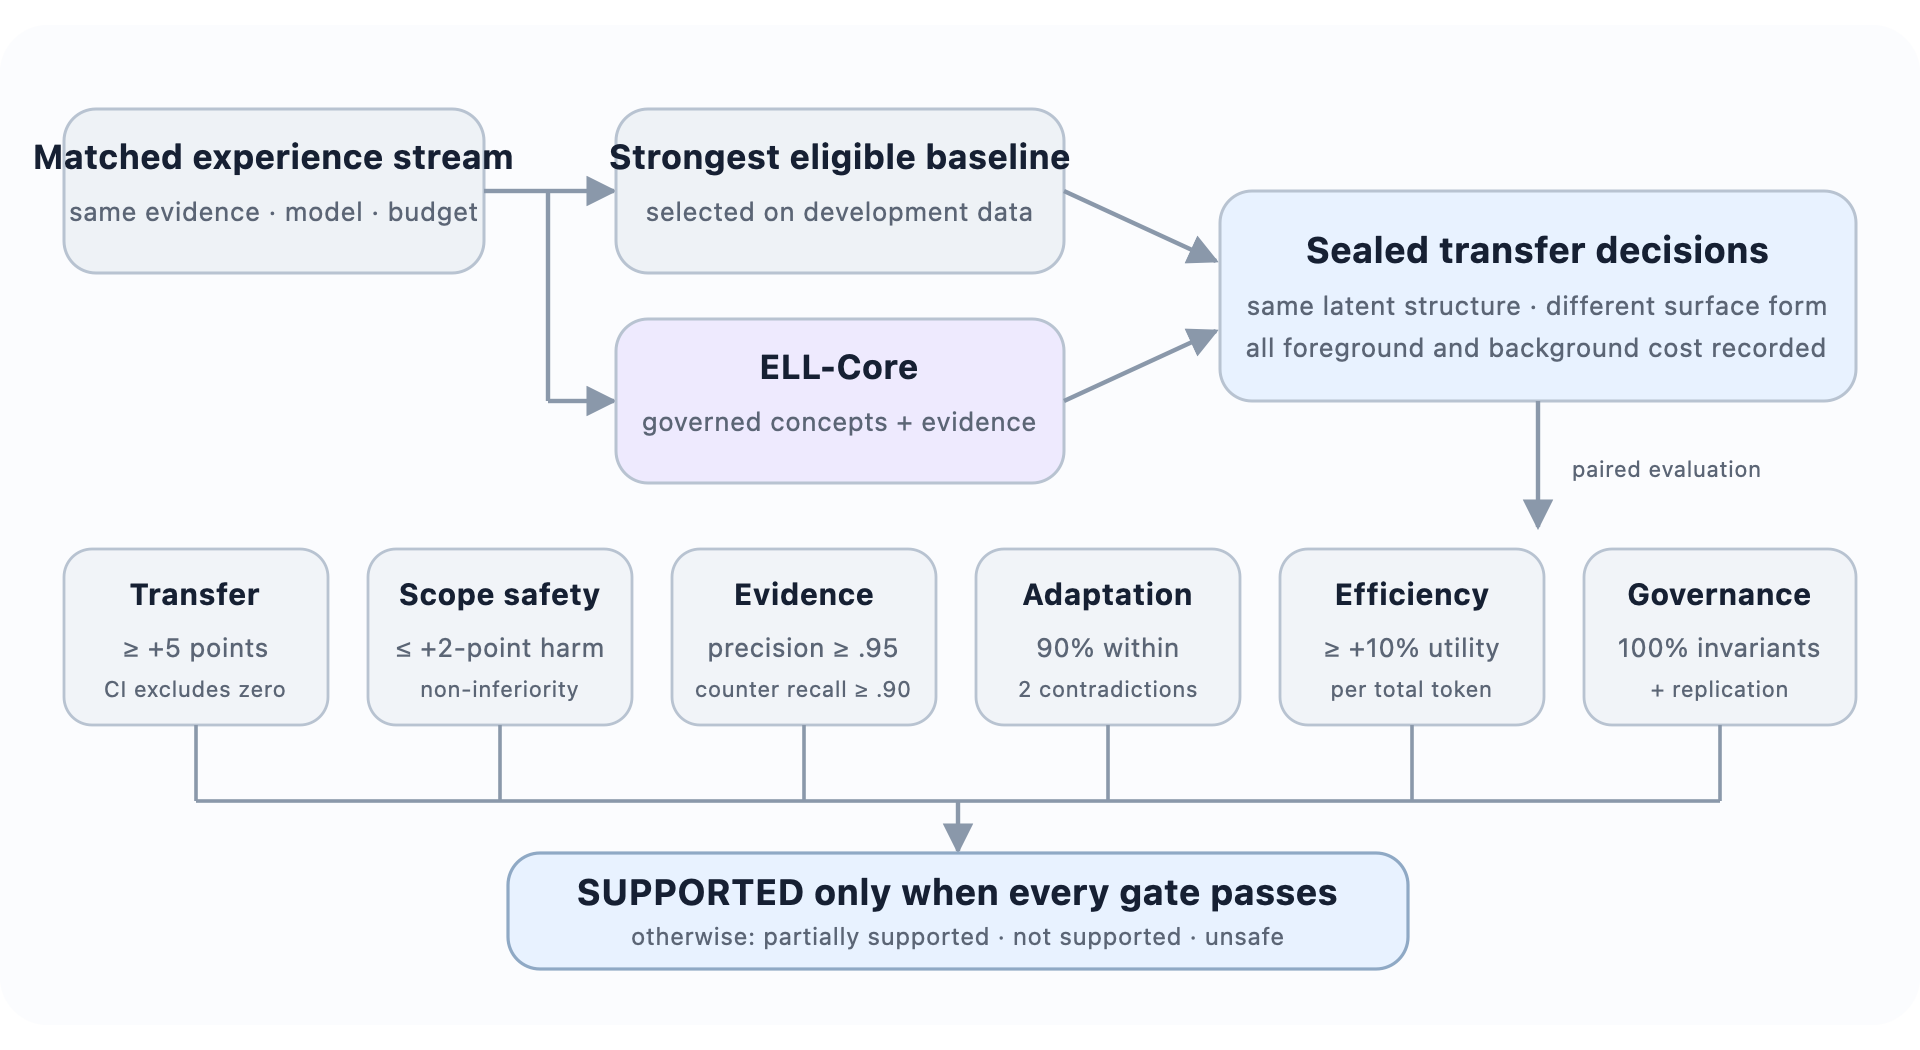
\includegraphics[keepaspectratio]{chapters/assets/diagrams/success-gates.png}}

}

\caption{\textbf{The ELL decision rule.} The same stream and model
conditions feed the strongest eligible baseline and ELL-Core. A positive
transfer result is reported as supported only when every guardrail also
passes.}

\end{figure}%

{\def\LTcaptype{none} % do not increment counter
\begin{longtable}[]{@{}
  >{\raggedright\arraybackslash}p{(\linewidth - 4\tabcolsep) * \real{0.3333}}
  >{\raggedright\arraybackslash}p{(\linewidth - 4\tabcolsep) * \real{0.3333}}
  >{\raggedright\arraybackslash}p{(\linewidth - 4\tabcolsep) * \real{0.3333}}@{}}
\toprule\noalign{}
\begin{minipage}[b]{\linewidth}\raggedright
Gate
\end{minipage} & \begin{minipage}[b]{\linewidth}\raggedright
Measure
\end{minipage} & \begin{minipage}[b]{\linewidth}\raggedright
Pass rule
\end{minipage} \\
\midrule\noalign{}
\endhead
\bottomrule\noalign{}
\endlastfoot
Primary transfer & Paired task-success difference on structurally
related, lexically distant sealed cases & Point estimate at least
\textbf{+5 percentage points} over the strongest eligible baseline and
the paired 95\% confidence interval excludes zero \\
Unsupported generalisation & Decisions that apply a concept outside its
gold or adjudicated scope & Upper bound of the paired 95\% confidence
interval is less than a \textbf{+2-point non-inferiority margin}
relative to the comparator \\
Evidence quality & Precision of cited support and recall of material
counterevidence & Support precision at least \textbf{0.95} and
counterevidence recall at least \textbf{0.90} on the controlled
benchmark \\
Change adaptation & Delay after a gold change point or material
correction & At least \textbf{90\%} of affected concepts are contested
or revised within two relevant contradictory episodes; post-change
stale-guidance rate remains below \textbf{5\%} \\
Cost efficiency & Task utility divided by all amortised input and output
tokens & At least \textbf{10\% higher utility per 1,000 total tokens}
than the confirmatory comparator, including background work \\
Governance invariants & Workspace isolation, idempotency, lineage,
deletion and projection invalidation & \textbf{100\% pass} on
deterministic and adversarial contract tests; no observed
cross-workspace retrieval and no deleted evidence remaining reachable in
tested projections \\
Replication & Sensitivity to model and task family & Primary transfer
and unsupported-generalisation gates pass with two open model families;
the transfer direction is also positive on at least one external
cognitive or action benchmark \\
\end{longtable}
}

The benchmark sample size will be selected to provide at least 80\%
power for the five-point paired primary effect. Exact power assumptions,
exclusions, seeds, and analysis code will be committed before the sealed
run.

\section{Outcome labels}\label{outcome-labels}

\textbf{Supported.} Every gate passes. The paper may conclude that
ELL-Core provides evidence for a useful governed concept layer under the
tested conditions.

\textbf{Partially supported.} Transfer improves, but one or more safety,
adaptation, efficiency, governance, or replication gates fail. The paper
must name the failed gate and cannot recommend the full architecture for
deployment.

\textbf{Not supported.} The primary transfer gate fails, or the
strongest simple baseline matches ELL at lower cost. Work should then
focus on the winning simpler method, such as evidence-grounded
retrieval, agent-controlled search, or direct insights.

\textbf{Unsafe.} A governance invariant fails. The affected
configuration is ineligible for deployment regardless of average task
performance.

\section{Product success is a later
claim}\label{product-success-is-a-later-claim}

After the confirmatory result, a product study may test whether people
experience less repetition, better shorthand understanding, timely
context, rapid correction, and trustworthy control. Product success
requires blinded task evaluation and user research; it cannot be
inferred from synthetic benchmark accuracy. The word \emph{intuition}
remains a product-level description of these behaviours, not the primary
scientific outcome.

\section{Explicit rejection
conditions}\label{explicit-rejection-conditions}

The central approach is weakened or rejected if:

\begin{itemize}
\tightlist
\item
  direct insight extraction or agent-controlled flat memory matches ELL
  at lower cost;
\item
  concept metrics improve without improving held-out decisions;
\item
  concept packets omit exceptions that raw episode retrieval preserves;
\item
  gains disappear under equal total-compute accounting;
\item
  revision causes unstable concept churn or slow recovery after change;
\item
  results depend on one model family, one generator, or one evaluator;
\item
  the system cannot invalidate derived state after deletion; or
\item
  outcome feedback strengthens concepts without independent evidence
  that their use helped.
\end{itemize}

Negative results remain valuable. They can show that explicit concepts
are unnecessary for some task classes, that consolidation should be
triggered only by failures, or that governed evidence retrieval is more
useful than concept formation.

\bookmarksetup{startatroot}

\chapter{ELL Research and Implementation
Plan}\label{ell-research-and-implementation-plan}

\section{Planning rule}\label{planning-rule}

ELL is built in evidence-producing vertical slices. Each phase must
leave a reproducible artefact, an exit report, and a go, revise, or stop
decision. The paper repository remains publication-first; executable
packages may be versioned separately and linked by immutable release
identifiers so implementation churn does not obscure the manuscript.

\section{Phase 0 --- Freeze the research
contract}\label{phase-0-freeze-the-research-contract}

Deliverables:

\begin{itemize}
\tightlist
\item
  publish paper v0.6 with the narrowed ELL-Core boundary;
\item
  freeze the primary estimand, success gates, baseline eligibility
  rules, and cost-accounting schema;
\item
  publish the source, episode, reflection, concept, evidence-link,
  application, outcome, and audit schemas as specifications;
\item
  publish worked examples for support, counterevidence, revision,
  deletion, and unsafe retrieval.
\end{itemize}

Exit criterion: an independent reader can identify exactly what result
would support or reject ELL and can rebuild the HTML and PDF from the
same sources.

\section{Phase 1 --- Build the benchmark before
ELL}\label{phase-1-build-the-benchmark-before-ell}

Deliverables:

\begin{itemize}
\tightlist
\item
  implement deterministic latent-pattern streams with paraphrase,
  distractors, exceptions, correlated evidence, change points, delayed
  outcomes, permissions, and deletion events;
\item
  create chronological train, development, and sealed test partitions;
\item
  implement immutable run manifests and application receipts;
\item
  implement no-memory, maximum-context, BM25, exact-vector, fused
  retrieval, rolling-summary, and direct-insight baselines;
\item
  run a development-only power analysis and freeze the sealed
  configuration.
\end{itemize}

Exit criterion: two clean-machine runs reproduce the same dataset hashes
and deterministic baseline metrics, and stochastic conditions reproduce
within declared intervals. If the benchmark cannot distinguish
known-good from deliberately broken policies, stop and repair the
benchmark.

\section{Phase 2 --- Implement deterministic
ELL-Core}\label{phase-2-implement-deterministic-ell-core}

Deliverables:

\begin{itemize}
\tightlist
\item
  implement typed boundary schemas, an in-memory append-only store,
  deterministic identifiers, and an evidence ledger;
\item
  implement concept lifecycle transitions, valid-time and observed-time
  handling, idempotency, workspace isolation, and deletion invalidation
  without an LLM;
\item
  use fixture reflections and concepts to test the entire
  application--outcome loop;
\item
  add property and adversarial tests for lineage, retries, corrections,
  tombstones, and cross-workspace access.
\end{itemize}

Exit criterion: all governance invariants pass and every derived object
resolves to permitted source spans. No graph database, hosted memory
provider, approximate vector index, or learned policy is permitted in
this phase.

\section{Phase 3 --- Add model-assisted reflection and
consolidation}\label{phase-3-add-model-assisted-reflection-and-consolidation}

Deliverables:

\begin{itemize}
\tightlist
\item
  add structured-generation adapters for at least two open model
  families;
\item
  quarantine generated candidates before deterministic validation and
  commit;
\item
  implement reflection, counterevidence search, concept proposal, merge,
  split, revision, and evidence restoration;
\item
  run same-model, cross-model, deterministic-validator, and human-review
  conditions;
\item
  execute the preregistered component ablations on development data,
  then freeze prompts and policies.
\end{itemize}

Exit criterion: the sealed ELL-Core comparison can run without manual
intervention and emits complete evidence, decision, outcome, and cost
traces. A failed governance invariant blocks the sealed run.

\section{Phase 4 --- Run the confirmatory
study}\label{phase-4-run-the-confirmatory-study}

Deliverables:

\begin{itemize}
\tightlist
\item
  select the strongest eligible baseline using development data only;
\item
  execute the sealed comparison once per frozen model and seed
  condition;
\item
  publish all gate results, confidence intervals, exclusions, failures,
  and raw receipts;
\item
  issue a supported, partially supported, not supported, or unsafe
  verdict using Section 11 without post-hoc threshold changes.
\end{itemize}

Exit criterion: the result can be reproduced from a tagged benchmark,
implementation, configuration, and paper release. If the primary gate
fails, stop concept-layer expansion and investigate the winning simpler
baseline.

\section{Phase 5 --- Evaluate persistence and replaceable
substrates}\label{phase-5-evaluate-persistence-and-replaceable-substrates}

This phase begins only if Phase 4 supports continued work.

Deliverables:

\begin{itemize}
\tightlist
\item
  add SQLite plus full-text search as the first durable local adapter;
\item
  compare exact vectors, HNSW, and TurboVec under identical candidate
  and permission filters;
\item
  reproduce selected Hindsight, TencentDB Agent Memory, Mem0,
  Zep/Graphiti, and Letta conditions through narrow adapters where their
  public interfaces and licences permit;
\item
  verify rebuildability, crash recovery, deletion propagation, provider
  egress controls, and cost accounting.
\end{itemize}

Exit criterion: replacing a substrate does not change canonical
identity, lifecycle, permissions, or evaluation semantics, and any
performance claim is tied to a reproducible adapter version.

\section{Phase 6 --- External validity and product
pilot}\label{phase-6-external-validity-and-product-pilot}

Deliverables:

\begin{itemize}
\tightlist
\item
  run LoCoMo-Plus and at least one memory-dependent action benchmark
  such as Mem2ActBench or MemoryArena;
\item
  complete blinded human evaluation of concept support, scope,
  usefulness, and correction;
\item
  test shorthand, proactive relevance, correction, explanation, and
  control in a consented small pilot;
\item
  measure total system cost, user-perceived intrusiveness, and failure
  recovery.
\end{itemize}

Exit criterion: the transfer direction survives at least one external
benchmark, no mandatory safety gate regresses, and users can inspect,
correct, scope, and delete learned state. Only then should a product
client or broader connector programme be planned.

\section{Deferred research tracks}\label{deferred-research-tracks}

Learned memory-operation policies, autonomous skill evolution,
experience graphs, neural or parametric memory, multimodal capture,
sync, and hosted memory services remain separate experiments. They are
not bundled into ELL-Core and must each justify themselves through a
preregistered incremental comparison.

\bookmarksetup{startatroot}

\chapter{Deferred Experience Learning Layer
Expansion}\label{deferred-experience-learning-layer-expansion}

The research architecture above asks whether evidence-grounded concepts
improve transfer and future behaviour. This chapter records the broader
product and research horizon, not the Phase 1 implementation plan. None
of these extensions enters the confirmatory comparison unless ELL-Core
first clears the gates in Section 11.

The expanded architecture generalises the initial scaffold into an open,
local-first experience-learning layer usable by people, applications,
and AI agents. It does not replace the original empirical question.

L is not primarily a chatbot, note-taking application, Zettelkasten,
vector database, or graph visualisation. Its north star is to give any
AI a natural, evolving intuition about the user or
organisation---grounded in experience, economical to use, sensitive to
change, explainable when inspected, and always under user control. Its
learning loop captures an experience, preserves its source, extracts
typed candidates, decides under deterministic policy what may become
durable, consolidates related memories without losing contradictions,
retrieves the smallest useful context, observes outcomes, and revises
future behaviour. Models interpret meaning and propose. Deterministic
services validate, authorize, version, and commit.

Intuition is an emergent capability of this loop, not another row type
or a claim that the system resembles a person. Evidence-grounded
compression, prediction, association, relevance selection, temporal
adaptation, and outcome feedback should together support shorthand,
proactive just-in-time context, useful generalisation, rapid correction,
change detection, calibrated uncertainty, and optional explanation. The
delivery object is a compact intuition packet with sufficient evidence
and uncertainty to be useful, plus stable references for deeper
inspection.

\section{System layers and technology
boundaries}\label{system-layers-and-technology-boundaries}

The expanded architecture has three independently evolvable layers:

\begin{itemize}
\tightlist
\item
  input and capture adapters turn conversations, recordings, documents,
  application events, and future connectors into immutable source
  artifacts, normalized events, and bounded episodes;
\item
  memory and retrieval infrastructure provides replaceable persistence,
  search, association, graph, vector, or hosted-memory projections;
\item
  the canonical learning layer evaluates evidence, maintains temporal
  and probabilistic hypotheses, governs durable concepts, records
  applications and outcomes, and controls revision, contradiction, and
  forgetting.
\end{itemize}

None of these layers is implemented in the current paper repository.
SQLite, hosted memory services, vector indexes, and graphs remain
candidate adapters or projections to integrate and compare. The
canonical learning layer is specified through proposed lifecycle
contracts, but those contracts are not yet an operational closed
learning loop. This distinction prevents an external memory system from
silently becoming L's truth or policy authority when implementation
begins.

The proposed direction is immutable evidence plus dynamic, temporal,
probabilistic concepts and hypotheses. Extraction, association,
consolidation, retrieval, and forgetting policies should be pluggable
and may become model-driven or learned. Their proposals remain subject
to deterministic provenance, permissions, workspace isolation, deletion,
schema, and canonical commit governance. No fixed graph, vector method,
note-linking scheme, or model family is selected as the final
architecture before the success criteria and ablations in Section 7 are
run.

\section{Plural memory semantics}\label{plural-memory-semantics}

The v0.1 paper distinguishes episodes, reflections, concepts,
applications, and outcomes. The broader ELL architecture retains these
objects while distinguishing additional memory semantics that have
different authority, lifetime, and retrieval rules:

\begin{itemize}
\tightlist
\item
  source memory preserves immutable artifacts and exact addressable
  spans;
\item
  working memory holds expiring state for the current task or
  conversation;
\item
  episodic memory represents bounded experiences, decisions, actions,
  and outcomes;
\item
  semantic memory represents temporal assertions rather than timeless
  key-value pairs;
\item
  preference memory represents scoped choices, exceptions, strength, and
  explicitness;
\item
  procedural memory represents versioned workflows, preconditions,
  approvals, evidence, and rollback;
\item
  prospective memory represents commitments, reminders, deadlines, and
  unresolved threads;
\item
  relational memory represents evidence-backed temporal edges;
\item
  reflective memory records uncertainty, freshness, usefulness,
  contradictions, and knowledge gaps;
\item
  policy memory defines retention, consent, provider, sharing, and
  deletion boundaries and is never ordinary model context.
\end{itemize}

These forms may share infrastructure, but they must not be flattened
into one untyped table with identical lifecycle semantics. The useful
layer is the explainable connection between evidence and future
behaviour, not a decorative node cloud.

\section{Source, event, and episode
boundary}\label{source-event-and-episode-boundary}

All provider connectors terminate at a common normalization boundary. An
immutable SourceArtifact preserves source identity, checksums,
timestamps, sensitivity, consent, and stable spans. Normalized
ExperienceEvents represent user messages, assistant messages, tool calls
and results, file changes, decisions, feedback, and external events. One
or more events form a bounded Episode containing inputs, responses,
actions, observations, and outcomes.

Stable deterministic identifiers make ingestion rerunnable. The same
connector, external reference, source version, and source event produce
the same domain IDs. Conversation exports, tool traces, calendar
records, or future connectors can therefore be replaced without placing
their schemas inside reflection, consolidation, policy, or retrieval
services.

\section{Governed candidate and commit
path}\label{governed-candidate-and-commit-path}

\begin{figure}[H]

{\centering \pandocbounded{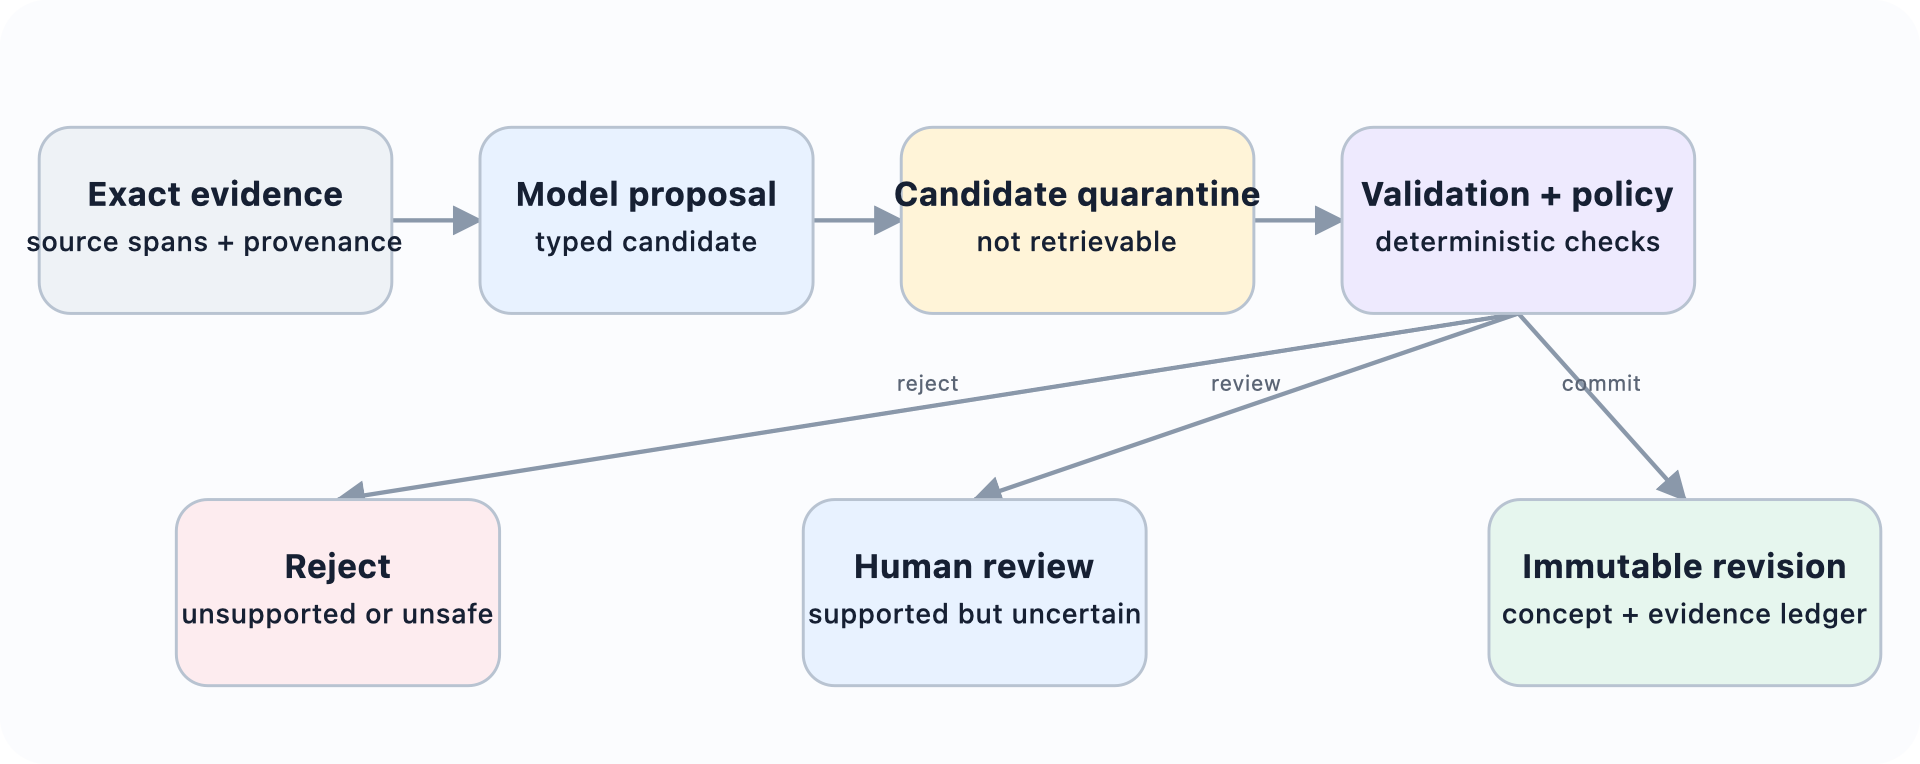
\includegraphics[keepaspectratio]{chapters/assets/diagrams/governed-commit.png}}

}

\caption{\textbf{Models interpret; deterministic code governs.}
Generated interpretations enter quarantine. Schema validation and
deterministic policy decide whether they are rejected, reviewed, or
committed.}

\end{figure}%

A model response is untrusted structured input. It enters a
CandidateMemory quarantine and cannot participate in normal retrieval.
Deterministic validation checks the schema, cited source and span
existence, workspace access, sensitivity inheritance, temporal fields,
allowed predicates, and referenced memories. Policy then selects one of
three initial outcomes:

\begin{itemize}
\tightlist
\item
  explicit user statements, corrections, and user-confirmed candidates
  may commit after validation;
\item
  supported ordinary inferences and inferred procedures wait for review;
\item
  unsupported non-explicit claims and sensitive model inferences are
  rejected.
\end{itemize}

The commit service is the sole canonical writer. It uses idempotency
keys and optimistic concurrency, writes an immutable revision, appends a
content-minimized audit event, and schedules disposable projections. A
correction creates a new memory and closes the validity of the
superseded revision. It never rewrites history. A lower-authority
inference cannot supersede explicit user evidence.

\section{Policy-bound evidence
retrieval}\label{policy-bound-evidence-retrieval}

Retrieval is a typed service rather than direct database or vector-index
access. A request includes actor, purpose, workspace, scope, allowed
memory types, maximum sensitivity, evidence preference, and a fixed
context budget. Authorization and lifecycle filtering happen before
relevance ranking. Superseded, forgotten, expired, cross-workspace, and
sensitivity-incompatible records do not enter ordinary results.

Candidate generation may combine lexical search, vectors, relation
neighbourhoods, time, pinning, procedures, and later learned rerankers.
Exact-vector, HNSW, graph, and hosted memory adapters remain replaceable
projections to benchmark; no index or provider is canonical memory. The
response is an EvidencePacket, presented at the application boundary as
an intuition packet, containing selected current claims, scoped
preferences, episodes, procedures, commitments, citations, selection
explanations, uncertainty, and known material contradictions. A compact
concept never becomes a naked instruction detached from its source.

Concrete comparison adapters may wrap Hindsight's structured networks,
Graphiti/Zep temporal graphs, Mem0 extraction and retrieval, Letta-style
context management, or TencentDB Agent Memory's layered Chat Memory,
Skill, Wiki, and CodeGraph assets. Exact search, HNSW, and TurboVec
remain alternative retrieval projections beneath the same policy filter.
Learned-policy adapters may later implement AgeMem-style tool actions,
AtomMem-style atomic operations, or MemSkill-style evolving routines.
Experience and skill adapters may provide EXG-style graphs,
ReasoningBank-style strategies, or lifecycle-managed skill candidates.
Neural accelerators may provide Titans-, HOPE-, or TMEM-style state. In
every case, the adapter returns candidates or acceleration state;
canonical source, concept, application, outcome, and deletion records
remain governed by ELL.

\section{Local-first and provider-neutral
topology}\label{local-first-and-provider-neutral-topology}

\begin{figure}[H]

{\centering \pandocbounded{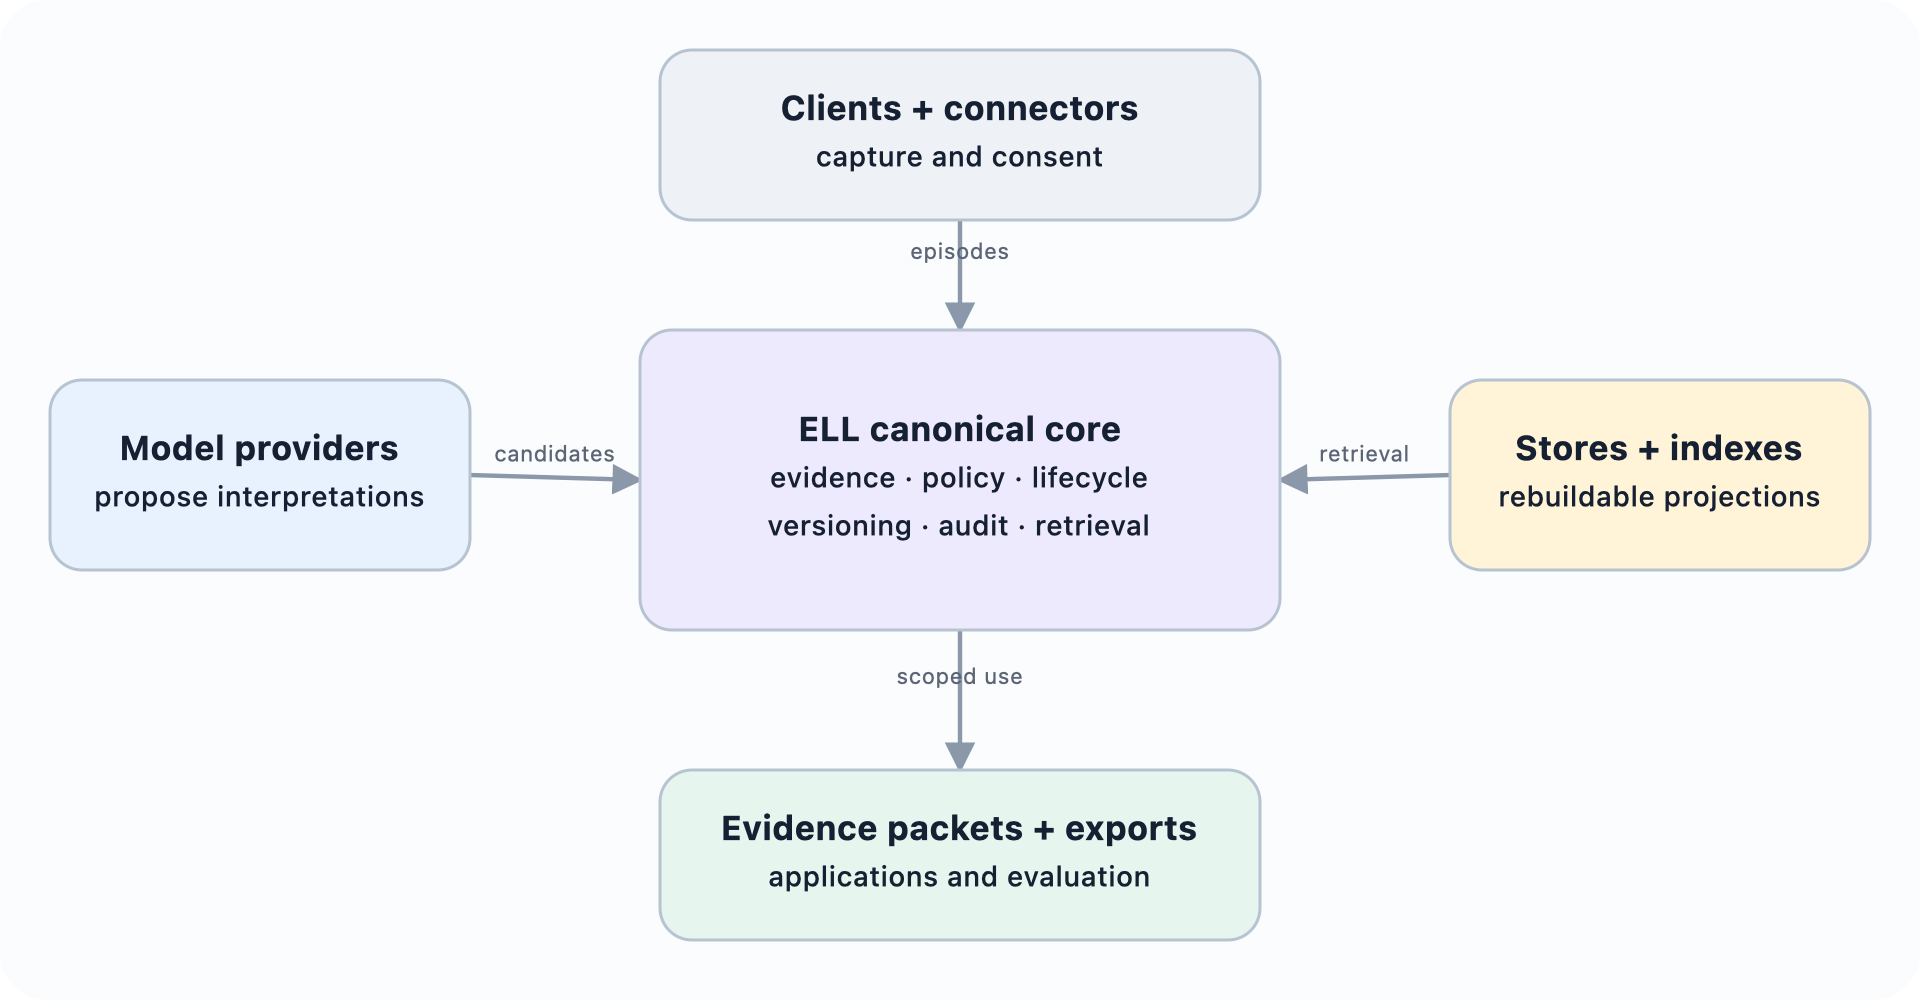
\includegraphics[keepaspectratio]{chapters/assets/diagrams/provider-neutral.png}}

}

\caption{\textbf{Canonical learning stays provider-neutral.} Clients,
model providers, stores, and indexes are replaceable adapters. Canonical
identity, evidence, policy, lifecycle, and audit remain inside ELL.}

\end{figure}%

A complete usable state can live on one device. Network absence must not
prevent capture, browsing, correction, or lexical retrieval. Remote
processing visibly degrades to local processors or queued work. A
practical reference adapter may use SQLite, content-addressed encrypted
files, FTS5, and a replaceable vector index, but these technologies do
not define the domain.

Four authentication concerns remain separate: L user identity, workspace
authorization, model-provider credentials, and connector grants. A model
adapter may call a provider API; a client or agent may call L through a
narrow protocol; or L may export a scoped context bundle. Provider
credentials never define L identity, canonical records, or access
policy.

Forgetting immediately excludes a record, writes a tombstone, removes
projections, and triggers evidence-aware invalidation. Sync must not
resurrect tombstoned content. Sensitive trait inference is disabled for
automatic durable learning. Imported documents are untrusted content,
never system instructions. Secrets do not enter prompts, canonical
memory, exports, analytics, or logs.

\bookmarksetup{startatroot}

\chapter{Research Artifact Status}\label{research-artifact-status}

The repository is currently a publication artifact, not an executable
ELL implementation. This boundary keeps the architecture, hypotheses,
and planned contracts inspectable without presenting unvalidated code as
evidence for H1-H6.

\section{Canonical and generated
editions}\label{canonical-and-generated-editions}

The Quarto Markdown chapters are the sole canonical source. A single
\texttt{quarto\ render} derives the multi-page HTML reading edition and
the downloadable PDF. Quarto provides navigation, search, section
numbering, cross-format links, and publication metadata. Generated
output is ignored by Git and rebuilt locally or by the GitHub publishing
workflow, keeping ordinary paper edits small and reviewable.

\section{Synthetic lifecycle
examples}\label{synthetic-lifecycle-examples}

The repository includes a small synthetic JSONL collection covering
explicit scoped preferences, single-event inference, unsupported claims,
sensitive inference, explicit correction, material contradiction,
temporal change, Dutch evidence, and prompt injection embedded in
imported content. These cases make proposed policy outcomes concrete for
readers. They are examples, not a validated benchmark, and no empirical
result is inferred from them.

\section{Deliberately deferred
implementation}\label{deliberately-deferred-implementation}

Typed runtime schemas, a governed commit kernel, storage adapters, model
providers, evaluation code, and product clients are not part of this
paper repository. Adding them should happen only with a documented
evaluation contract and tests that can support any corresponding
implementation claim. Until then, the interfaces and algorithms in
Sections 5 and 6 are specifications.

\section{Remaining gates}\label{remaining-gates}

The next research step is the controlled benchmark: deterministic
experience streams, sealed evaluation partitions, policy sweeps,
application receipts, and reproducible comparisons with episode
retrieval, rolling summaries, and direct insight extraction. The
strongest eligible baseline will be selected on development data before
ELL-Core is evaluated on the sealed partition. A later reference
implementation must also demonstrate persistent-store rebuilds, deletion
propagation through projections, provider egress enforcement, job
recovery, and lifecycle correctness before it can count as evidence for
H1-H6.

The project does not advance merely because an implementation exists. It
advances when the primary transfer result and every mandatory guardrail
in Section 11 pass. If a simpler approach matches ELL at lower cost, the
research plan explicitly adopts that simpler method and records the
concept-layer hypothesis as unsupported for the tested conditions.

\bookmarksetup{startatroot}

\chapter{Conclusion}\label{conclusion}

The Experience Learning Layer begins from a simple distinction: access
to old experience is not the same as learning from it. Current research
already demonstrates reflection, dynamic memory organisation, schema
induction, concept graphs, and semantic or procedural abstraction. The
next useful contribution is therefore a stricter account of how an
abstraction earns trust, remains connected to evidence, changes when
challenged, and improves future behaviour.

ELL proposes an explicit path from episodes to provisional reflections,
from reflections to versioned concepts, and from concepts to measured
applications and outcomes. The architecture preserves both support and
counterevidence, treats scope and temporal validity as first-class
fields, and makes revision reversible and auditable. Its value will be
determined empirically, not by the plausibility of the design.

The practical expression of that hypothesis is economical, timely
context that helps an AI understand shorthand and adapt to change
without hiding where its guidance came from. The scientific claim is
narrower: under matched models, streams, and total compute, ELL-Core
must improve sealed structurally distant transfer by at least five
percentage points over the strongest eligible baseline while passing
every safety, evidence, adaptation, cost, governance, and replication
gate. The term \emph{intuition} is deferred to later product research.

The project is open by default. The paper, diagrams, synthetic examples,
and reproducible reading editions make the proposal easy to inspect,
criticise, and extend. The immediate next step is the benchmark, not a
product or a more elaborate architecture. If direct insight extraction,
agent-controlled flat memory, or evidence-grounded retrieval matches ELL
at lower cost, that result should replace the present design rather than
be explained away.

\bookmarksetup{startatroot}

\chapter*{Acknowledgements}\label{acknowledgements}
\addcontentsline{toc}{chapter}{Acknowledgements}

\markboth{Acknowledgements}{Acknowledgements}

This working draft was developed as part of the open Experience Learning
Layer project. Future versions will list contributors according to
documented authorship and contribution criteria.

\bookmarksetup{startatroot}

\chapter*{References}\label{references}
\addcontentsline{toc}{chapter}{References}

\markboth{References}{References}

Alchourrón, Carlos E., Peter Gärdenfors, and David Makinson. 1985. `On
the Logic of Theory Change: Partial Meet Contraction and Revision
Functions'. Journal of Symbolic Logic 50 (2): 510--30.
https://doi.org/10.2307/2274239.

Bartlett, Frederic C. 1932. Remembering: A Study in Experimental and
Social Psychology. Cambridge University Press.

Behrouz, Ali, Meisam Razaviyayn, Peilin Zhong, and Vahab Mirrokni. 2025.
`Nested Learning: The Illusion of Deep Learning Architectures'.
https://arxiv.org/abs/2512.24695.

Behrouz, Ali, Peilin Zhong, and Vahab Mirrokni. 2025. `Titans: Learning
to Memorize at Test Time'. https://arxiv.org/abs/2501.00663.

Chhikara, Prateek, Dev Khant, Saket Aryan, Taranjeet Singh, and Deshraj
Yadav. 2025. `Mem0: Building Production-Ready AI Agents with Scalable
Long-Term Memory'. https://arxiv.org/abs/2504.19413.

Chen, Zhikai, Jialiang Gu, Junyu Yin, Xianxuan Long, Shenglai Zeng,
Xiaoze Liu, Kai Guo, Keren Zhou, and Jiliang Tang. 2026. `Exploring
Cross-Scenario Generality of Agentic Memory Systems: Diagnostics and a
Strong Baseline'. https://arxiv.org/abs/2606.04315.

Clifford, James, and Tomas Isakowitz. 1992. `On the Semantics of
Transaction Time and Valid Time in Bitemporal Databases'. NYU Working
Paper IS-92-42. https://ssrn.com/abstract=1289024.

de Kleer, Johan. 1986. `An Assumption-Based TMS'. Artificial
Intelligence 28 (2): 127--62.
https://doi.org/10.1016/0004-3702(86)90080-9.

Doyle, Jon. 1979. `A Truth Maintenance System'. Artificial Intelligence
12 (3): 231--72. https://doi.org/10.1016/0004-3702(79)90008-0.

Fei, Tianxiang, Mingyang Song, Mao Zheng, and Xiang Yu. 2026. `Memory
Beyond Recall: A Dual-Process Cognitive Memory System for Self-Evolving
LLM Agents'. https://arxiv.org/abs/2606.09483.

He, Zexue, Yu Wang, Churan Zhi, Yuanzhe Hu, Tzu-Ping Chen, Lang Yin, Ze
Chen, et al.~2026. `MemoryArena: Benchmarking Agent Memory in
Interdependent Multi-Session Agentic Tasks'.
https://arxiv.org/abs/2602.16313.

Hu, Yuanzhe, Yu Wang, and Julian McAuley. 2025. `Evaluating Memory in
LLM Agents via Incremental Multi-Turn Interactions'.
https://arxiv.org/abs/2507.05257.

Hu, Qisheng, Quanyu Long, and Wenya Wang. 2026. `When Continual Learning
Moves to Memory: A Study of Experience Reuse in LLM Agents'.
https://arxiv.org/abs/2604.27003.

Hu, Sen, Yuxiang Wei, Jiaxin Ran, Zhiyuan Yao, Xueran Han, Huacan Wang,
Ronghao Chen, and Lei Zou. 2026. `Does Memory Need Graphs? A Unified
Framework and Empirical Analysis for Long-Term Dialog Memory'. In
Proceedings of the 64th Annual Meeting of the Association for
Computational Linguistics, 26758--82.
https://aclanthology.org/2026.acl-long.1232/.

Huo, Yupeng, Yaxi Lu, Zhong Zhang, Haotian Chen, and Yankai Lin. 2026.
`AtomMem: Learnable Dynamic Agentic Memory with Atomic Memory
Operation'. https://arxiv.org/abs/2601.08323.

Jin, Yuxin, Siyuan Zhang, Hanchen Wang, Lu Qin, Ying Zhang, and Wenjie
Zhang. 2026. `EXG: Self-Evolving Agents with Experience Graphs'.
https://arxiv.org/abs/2605.17721.

Jiang, Eric Hanchen, Zhi Zhang, Yuchen Wu, Levina Li, Dong Liu, Xiao
Liang, Rui Sun, Yubei Li, Edward Sun, Haozheng Luo, Zhaolu Kang, Aylin
Caliskan, Kai-Wei Chang, and Ying Nian Wu. 2026. `Memory as a Controlled
Process: Learned Adaptive Memory Management for LLM Agents'.
https://arxiv.org/abs/2607.13591.

Kumaran, Dharshan, Demis Hassabis, and James L. McClelland. 2016. `What
Learning Systems Do Intelligent Agents Need?

Complementary Learning Systems Theory Updated'. Trends in Cognitive
Sciences 20 (7): 512--34. https://doi.org/10.1016/j.tics.2016.05.004.

Letta. 2026. `Letta: Platform for Building Stateful Agents'. Software
repository. https://github.com/letta-ai/letta.

Latimer, Christopher, Nicolò Boschi, Andrew Neeser, Chris Bartholomew,
Gaurav Srivastava, Xuan Wang, and Naren Ramakrishnan. 2026. `Hindsight:
Structured Agent Memory that Retains, Recalls, and Reflects'. In
Proceedings of the 64th Annual Meeting of the Association for
Computational Linguistics: System Demonstrations, 275--85.
https://doi.org/10.18653/v1/2026.acl-demo.27.

Lebo, Timothy, Satya Sahoo, and Deborah McGuinness, eds.~2013. `PROV-O:
The PROV Ontology'. W3C Recommendation. https://www.w3.org/TR/prov-o/.

Li, Yifei, Weidong Guo, Lingling Zhang, Rongman Xu, Muye Huang, Hui Liu,
Lijiao Xu, Yu Xu, and Jun Liu. 2026. `LoCoMo-Plus: Beyond-Factual
Cognitive Memory Evaluation Framework for LLM Agents'. In Proceedings of
the 64th Annual Meeting of the Association for Computational
Linguistics, 25085--100. https://doi.org/10.18653/v1/2026.acl-long.1150.

Lin, Huawei, Peng Li, Jie Song, Fuxin Jiang, and Tieying Zhang. 2026.
`MUSE-Autoskill: Self-Evolving Agents via Skill Creation, Memory,
Management, and Evaluation'. https://arxiv.org/abs/2605.27366.

Luo, Jinghao, Yuchen Tian, Chuxue Cao, Ziyang Luo, Hongzhan Lin, Kaixin
Li, Chuyi Kong, Ruichao Yang, and Jing Ma. 2026. `From Storage to
Experience: A Survey on the Evolution of LLM Agent Memory Mechanisms'.
In Findings of the Association for Computational Linguistics: ACL 2026,
41622--52. https://doi.org/10.18653/v1/2026.findings-acl.2069.

Maharana, Adyasha, Dong-Ho Lee, Sergey Tulyakov, Mohit Bansal, Francesco
Barbieri, and Yuwei Fang. 2024. `Evaluating Very Long-Term
Conversational Memory of LLM Agents'. In Proceedings of the 62nd Annual
Meeting of the Association for Computational Linguistics, 13851--70.
https://doi.org/10.18653/v1/2024.acl-long.747.

McClelland, James L., Bruce L. McNaughton, and Randall C. O'Reilly.
1995. `Why There Are Complementary Learning Systems in the Hippocampus
and Neocortex: Insights from the Successes and Failures of Connectionist
Models of Learning and Memory'.

Psychological Review 102 (3): 419--57.
https://doi.org/10.1037/0033-295X.102.3.419.

Packer, Charles, Sarah Wooders, Kevin Lin, Vivian Fang, Shishir G.
Patil, Ion Stoica, and Joseph E. Gonzalez. 2023. `MemGPT: Towards LLMs
as Operating Systems'. https://arxiv.org/abs/2310.08560.

Ouyang, Siru, Jun Yan, I-Hung Hsu, Yanfei Chen, Ke Jiang, Zifeng Wang,
Rujun Han, et al.~2026. `ReasoningBank: Scaling Agent Self-Evolving with
Reasoning Memory'. In International Conference on Learning
Representations. https://arxiv.org/abs/2509.25140.

Park, Joon Sung, Joseph C. O'Brien, Carrie J. Cai, Meredith Ringel
Morris, Percy Liang, and Michael S. Bernstein. 2023. `Generative Agents:
Interactive Simulacra of Human Behavior'. In Proceedings of the 36th
Annual ACM Symposium on User Interface Software and Technology, 1--22.
https://doi.org/10.1145/3586183.3606763.

Paul, Swarna Kamal, Shubhendu Sharma, and Nitin Sareen. 2026. `GAAMA:
Graph Augmented Associative Memory for Agents'.
https://arxiv.org/abs/2603.27910.

Rasmussen, Preston, Pavlo Paliychuk, Travis Beauvais, Jack Ryan, and
Daniel Chalef. 2025. `Zep: A Temporal Knowledge Graph Architecture for
Agent Memory'. https://arxiv.org/abs/2501.13956.

Ren, Tao, Weiyao Luo, Hui Yang, Rongzhi Zhu, Xiang Huang, Yuchuan Wu,
Bingxue Chou, et al.~2026. `Scaling Self-Evolving Agents via Parametric
Memory'. https://arxiv.org/abs/2606.04536.

Shinn, Noah, Federico Cassano, Edward Berman, Ashwin Gopinath, Karthik
Narasimhan, and Shunyu Yao. 2023. `Reflexion: Language Agents with
Verbal Reinforcement Learning'. In Advances in Neural Information
Processing Systems. Vol. 36. https://arxiv.org/abs/2303.11366.

Shen, Yiting, Kun Li, Wei Zhou, and Songlin Hu. 2026. `Mem2ActBench: A
Benchmark for Evaluating Long-Term Memory Utilization in Task-Oriented
Autonomous Agents'. In Proceedings of the 64th Annual Meeting of the
Association for Computational Linguistics, 8173--90.
https://doi.org/10.18653/v1/2026.acl-long.370.

Shukla, Navnit, Kamal Pandey, and Omsankar Tiwari. 2026. `TurboVec: A
Case Study in Cost-Efficient Private Retrieval for Enterprise RAG via
Codebook-Oblivious Quantization'. https://arxiv.org/abs/2607.16973.

Su, Miao, Yucan Guo, Zhongni Hou, Long Bai, Zixuan Li, Yufei Zhang,
Guojun Yin, et al.~2026. `Beyond Dialogue Time: Temporal Semantic Memory
for Personalized LLM Agents'. https://arxiv.org/abs/2601.07468.

Sumers, Theodore R., Shunyu Yao, Karthik Narasimhan, and Thomas L.
Griffiths. 2024. `Cognitive Architectures for Language Agents'.

Transactions on Machine Learning Research.
https://arxiv.org/abs/2309.02427.

Tan, Haoran, Zeyu Zhang, Chen Ma, Xu Chen, Quanyu Dai, and Zhenhua Dong.
2025. `MemBench: Towards More Comprehensive Evaluation on the Memory of
LLM-Based Agents'. In Findings of the Association for Computational
Linguistics: ACL 2025. https://arxiv.org/abs/2506.21605.

Tan, Zhen, Jun Yan, I-Hung Hsu, Rujun Han, Zifeng Wang, Long T. Le,
Yiwen Song, et al.~2025. `In Prospect and Retrospect: Reflective Memory
Management for Long-Term Personalized Dialogue Agents'. In Proceedings
of the 63rd Annual Meeting of the Association for Computational
Linguistics, 8416--39. https://doi.org/10.18653/v1/2025.acl-long.413.

TencentDB Agent Memory Team. 2026. `TencentDB Agent Memory'. Software
repository, accessed 9 August 2026.
https://github.com/TencentCloud/TencentDB-Agent-Memory.

Tulving, Endel. 1972. `Episodic and Semantic Memory'. In Organization of
Memory, edited by Endel Tulving and Wayne Donaldson, 381--403. Academic
Press.

Wang, Guanzhi, Yuqi Xie, Yunfan Jiang, Ajay Mandlekar, Chaowei Xiao,
Yuke Zhu, Linxi Fan, and Anima Anandkumar. 2023.

`Voyager: An Open-Ended Embodied Agent with Large Language Models'. In
Transactions on Machine Learning Research.
https://arxiv.org/abs/2305.16291.

Wang, Zora Zhiruo, Jiayuan Mao, Daniel Fried, and Graham Neubig. 2025.
`Agent Workflow Memory'. In Proceedings of the 42nd International
Conference on Machine Learning, 267:63897--911. Proceedings of Machine
Learning Research.

Wu, Di, Hongwei Wang, Wenhao Yu, Yuwei Zhang, Kai-Wei Chang, and Dong
Yu. 2025. `LongMemEval: Benchmarking Chat Assistants on Long-Term
Interactive Memory'. In International Conference on Learning
Representations. https://arxiv.org/abs/2410.10813.

Xu, Wujiang, Zujie Liang, Kai Mei, Hang Gao, Juntao Tan, and Yongfeng
Zhang. 2025. `A-MEM: Agentic Memory for LLM Agents'.

In Advances in Neural Information Processing Systems.
https://arxiv.org/abs/2502.12110.

Yang, Ke, Zixi Chen, Xuan He, Jize Jiang, Michel Galley, Chenglong Wang,
Jianfeng Gao, Jiawei Han, and ChengXiang Zhai. 2026.

`PlugMem: A Task-Agnostic Plugin Memory Module for LLM Agents'.
https://arxiv.org/abs/2603.03296.

Yu, Yi, Liuyi Yao, Yuexiang Xie, Qingquan Tan, Jiaqi Feng, Yaliang Li,
and Libing Wu. 2026. `Agentic Memory: Learning Unified Long-Term and
Short-Term Memory Management for Large Language Model Agents'.
https://arxiv.org/abs/2601.01885.

Zhang, Jiawen, Kejia Chen, Jiachen Ma, Yangfan Hu, Lipeng He, Yechao
Zhang, Jian Liu, Xiaohu Yang, Tianwei Zhang, and Ruoxi Jia. 2026.
`Beyond Similarity: Trustworthy Memory Search for Personal AI Agents'.
https://arxiv.org/abs/2606.06054.

Zhang, Haozhen, Quanyu Long, Jianzhu Bao, Tao Feng, Weizhi Zhang,
Haodong Yue, and Wenya Wang. 2026. `MemSkill: Learning and Evolving
Memory Skills for Self-Evolving Agents'.
https://arxiv.org/abs/2602.02474.

Zhao, Andrew, Daniel Huang, Quentin Xu, Matthieu Lin, Yong-Jin Liu, and
Gao Huang. 2024. `ExpeL: LLM Agents Are Experiential Learners'. In
Proceedings of the AAAI Conference on Artificial Intelligence,
38:19632--42. 17. https://doi.org/10.1609/aaai.v38i17.29936.

Zhong, Wanjun, Lianghong Guo, Qiqi Gao, He Ye, and Yanlin Wang. 2024.
`MemoryBank: Enhancing Large Language Models with Long-Term Memory'. In
Proceedings of the AAAI Conference on Artificial Intelligence,
38:19724--31. 17. https://doi.org/10.1609/aaai.v38i17.29946.

Zhou, Huichi, Siyuan Guo, Anjie Liu, Zhongwei Yu, Ziqin Gong, Bowen
Zhao, Zhixun Chen, et al.~2026. `Memento-Skills: Let Agents Design
Agents'. https://arxiv.org/abs/2603.18743.

Zep. 2026. `Graphiti: Build Real-Time Knowledge Graphs for AI Agents'.
Software repository. https://github.com/getzep/graphiti.




\end{document}
